\documentclass[10pt,xcolor=table]{beamer}

\usepackage{bbm}
\usepackage{textpos}
\usepackage{pgf,tikz}
\usepackage{graphicx}
% \usepackage{subfig}
\usepackage{forloop}
\usepackage[backend=bibtex]{biblatex}
\usepackage{animate}

\AtBeginSection[]
{
  \begin{frame}
    \frametitle{Three DPG Punchlines}
    \framesubtitle{\hspace{1ex}}
    \tableofcontents[currentsection,currentsubsection]
  \end{frame}
}
% \AtBeginSubsection[] {
%   \begin{frame}
%     \frametitle{Table of Contents}
%     \framesubtitle{\hspace{1ex}}
%     \tableofcontents[currentsection,currentsubsection]
%   \end{frame}
% }

\definecolor{utorange}{RGB}{203,96,21}
\definecolor{utblack}{RGB}{99,102,106}
\definecolor{utbrown}{RGB}{110,98,89}
\definecolor{utsecbrown}{RGB}{217,200,158}
\definecolor{utsecgreen}{RGB}{208,222,187}
\definecolor{utsecblue}{RGB}{127,169,174}

\mode<presentation>
{
  % \usetheme{Pittsburgh}
  \usetheme{Boadilla}
  \usefonttheme[onlymath]{serif}

  \setbeamercovered{invisible}
  \setbeamertemplate{navigation symbols}{}

  % Color Theme
    \setbeamercolor{normal text}{bg=white,fg=utblack}
  \setbeamercolor{structure}{fg=utorange}

  \setbeamercolor{alerted text}{fg=red!85!black}

  \setbeamercolor{item projected}{use=item,fg=black,bg=item.fg!35}

  \setbeamercolor*{palette primary}{use=structure,fg=white, bg=utorange}
  \setbeamercolor*{palette secondary}{use=structure,bg=utsecbrown}
  \setbeamercolor*{palette tertiary}{use=structure,bg=utsecgreen}
  \setbeamercolor*{palette quaternary}{use=structure,fg=structure.fg,bg=utsecblue}

  % \setbeamercolor*{frametitle}{use=structure,fg=utorange, bg=utsecbrown}
  \setbeamercolor*{framesubtitle}{fg=utbrown}

  \setbeamercolor*{block title}{parent=structure,fg=black,bg=utsecgreen}
  \setbeamercolor*{block body}{fg=black,bg=utblack!10}
  \setbeamercolor*{block title alerted}{parent=alerted text,bg=black!15}
  \setbeamercolor*{block title example}{parent=example text,bg=black!15}

  \setbeamerfont{framesubtitle}{size=\small}
}

\makeatletter
\setbeamertemplate{footline}
{
  \leavevmode%
    \hbox{%
      \begin{beamercolorbox}[wd=.333333\paperwidth,ht=2.25ex,dp=1ex,center]{author in head/foot}%
        \usebeamerfont{author in head/foot}\insertshortauthor%~~\beamer@ifempty{\insertshortinstitute}{}{(\insertshortinstitute)}
      \end{beamercolorbox}%
        \begin{beamercolorbox}[wd=.333333\paperwidth,ht=2.25ex,dp=1ex,center]{title in head/foot}%
        \usebeamerfont{title in head/foot}\insertshorttitle
        \end{beamercolorbox}%
        \begin{beamercolorbox}[wd=.333333\paperwidth,ht=2.25ex,dp=1ex,right]{date in head/foot}%
        \usebeamerfont{date in head/foot}\insertshortdate{}\hspace*{2em}
        \insertframenumber{} / \inserttotalframenumber\hspace*{2ex}
      \end{beamercolorbox}}%
        \vskip0pt%
}
\makeatother

\usepackage{kerkis}
\usepackage[T1]{fontenc}
\usepackage[protrusion=true,expansion=true]{microtype}
\usepackage{amsmath}


\renewcommand*{\thefootnote}{\fnsymbol{footnote}}

\let\oldfootnotesize\footnotesize
\renewcommand*{\footnotesize}{\oldfootnotesize\tiny}


\pgfdeclareimage[height=1.2cm]{utbig}{logos/UTWordmark}
\pgfdeclareimage[height=0.6cm]{ut}{logos/UTWordmark}

% -----PACKAGES
%\usepackage[shortend,titlenumbered]{algorithm2e}
%\usepackage{algorithmic}
%\usepackage[plain]{algorithm}
\usepackage{multicol}
\usepackage{color}
\usepackage{multirow}
\usepackage{fancybox}
%\usepackage{index}
\usepackage{varioref}
\usepackage{psfrag}
\usepackage{epsfig}
\usepackage{boxedminipage}
\usepackage{graphicx}
\usepackage{rotating}
\usepackage{amsmath}
\usepackage{amssymb}
%\usepackage{amsfont}
\usepackage{latexsym}
\usepackage{alltt}
%\usepackage[small,bf]{caption}
\usepackage{url}
%\usepackage{citesort}
%\usepackage{crop}
\usepackage{array}
\usepackage{subfigure}
\usepackage{dcolumn}

% -----SETLENGTH
%\setlength{\captionmargin}{20pt} 

% -----NEWCOMMANDS
\newcommand{\nc}{\newcommand}
\nc{\mathsm}[1]{\text{\small{$#1$}}}
\nc{\ubar}[1]{\underset{-}{#1}}
\nc{\optype}{\textrm}
\nc{\EQ}[1]{(\ref{eq:#1})}
\nc{\TAB}[1]{\ref{tab:#1}}
\nc{\FIG}[1]{\ref{fig:#1}}
\nc{\SEC}[1]{\ref{sec:#1}}
\nc{\ALG}[1]{\ref{alg:#1}}
\nc{\CHAP}[1]{\ref{chap:#1}}
\nc{\mtrx}[1]{\boldsymbol{\mathbf{#1}}}
\nc{\vctr}[1]{\boldsymbol{\mathbf{#1}}}
\nc{\grad}{\mbox{\boldmath$\nabla$}}
\nc{\gradient}{\textsl{grad}\,}
\nc{\hessian}{\textsl{grad\,}^2}
\nc{\ii}{\iota}
\nc{\dd}{d}
\nc{\ee}{\mathrm{e}}
\nc{\pdiv}[2]{\partial{#1}/\partial{#2}}
\nc{\dpdiv}[2]{\displaystyle{\frac{\partial{#1}}{\partial{#2}}}}
\nc{\ddiv}[2]{\displaystyle{\frac{\dd{#1}}{\dd{#2}}}}
\nc{\inpr}{\hspace{-1pt}\cdot\hspace{-1pt}}
\nc{\IR}{\mathbb{R}}
\nc{\IN}{\mathbb{N}}
\nc{\IZ}{\mathbb{Z}}
\nc{\IC}{\mathbb{C}}
\nc{\half}{\frac{1}{2}}
\nc{\shalf}{\scriptstyle{\half}} 
\nc{\ds}[1]{\displaystyle{#1}}
\nc{\ts}[1]{\textstyle{#1}}
\nc{\sign}{\optype{sign}}
\nc{\spr}{\optype{spr}}
\nc{\dist}{\optype{dist}}
\nc{\rank}{\optype{rank}}
\nc{\codim}{\optype{codim}}
\nc{\supp}{\optype{supp}}
\nc{\diag}{\optype{diag}}
\nc{\meas}{\optype{meas}}
\nc{\cond}{\optype{cond}}
\nc{\kernel}{\optype{kernel}}
\nc{\spa}{\optype{span}}
\nc{\order}{\mathcal{O}}
\nc{\Fr}{\mathrm{Fr}}
\nc{\Rey}{\mathrm{Re}}
\nc{\Ord}{O}
\nc{\ord}{o}
\nc{\st}{\:{:}\:}
\nc{\closure}[1]{\overline{#1}}
\nc{\emin}[1]{\emph{#1}\index{#1}\/}
\nc{\rmin}[1]{#1\index{{}@{#1}}}
\nc{\Laplace}{\Delta}
\nc{\ie}{i.e.}
\nc{\eg}{e.g.}
%\nc{\union}{\cup}
\nc{\Union}{\bigcup}
\nc{\lf}[1]{\mathsf{#1}}
\nc{\dbar}[1]{\bar{\bar{#1}}}
\nc{\ul}[1]{\underline{#1}}
\nc{\hpt}{\hspace{0.5pt}}
\nc{\E}[1]{\times{}10^{#1}}
\nc{\inp}[2]{\langle{#1},{#2}\rangle}
\nc{\tmpcommand}{}

% -----RENEWCOMMANDS
\renewcommand{\baselinestretch}{1}
\renewcommand{\exp}{\optype{exp}\,}
\renewcommand{\cosh}{\optype{cosh}\,}
\renewcommand{\tanh}{\optype{tanh}\,}
\renewcommand{\sinh}{\optype{sinh}\,}
\renewcommand{\div}[1]{\optype{div}\,{#1}}
\renewcommand{\half}{\mbox{$\frac{1}{2}$}}
%\renewcommand{\descriptionlabel}[1]{\hspace{\labelsep}\emph{#1}}

% -----ETC
\raggedbottom


\DeclareMathOperator{\curl}{\bf curl}
\DeclareMathOperator{\rot}{\rm curl}
\DeclareMathOperator{\divv}{\rm div}
\newcommand{\tro}{\gamma_0}
\newcommand{\trt}{\gamma_{\sft}}
\newcommand{\trn}{\gamma_{\sfn}}

\newcommand{\PT}{{\partial T}}
\newcommand{\bbN}{{\mathbb{N}}}
\newcommand{\bbP}{{\mathbb{P}}}

\newcommand{\scC}{{\mathscr{C}}}
\newcommand{\caD}{{\mathcal{D}}}
\newcommand{\caL}{{\mathcal{L}}}

\newcommand{\sfe}{{\mathsf{e}}}
\newcommand{\sff}{{\mathsf{f}}}
\newcommand{\sft}{{\boldsymbol{\mathsf{t}}}}
\newcommand{\sfn}{{\boldsymbol{\mathsf{n}}}}

%   Common caligraphic abbrevs
\newcommand{\BB}{\mathcal{B}}
\newcommand{\CC}{\mathcal{C}}
\newcommand{\DD}{\mathcal{D}}
\newcommand{\EE}{\mathcal{E}}
\newcommand{\FF}{\mathcal{F}}
\newcommand{\GG}{\mathcal{G}}
\newcommand{\II}{\mathcal{I}}
\newcommand{\JJ}{\mathcal{J}}
\newcommand{\KK}{\mathcal{K}}
\newcommand{\LL}{\mathcal{L}}
\newcommand{\OO}{\mathcal{O}}
\newcommand{\QQ}{\mathcal{Q}}
\newcommand{\RR}{\mathcal{R}}
\newcommand{\TT}{\mathcal{T}}


 %% JAY'S PREAMBLE
 %%========================

%   Math symbol definitions
\def\d{\partial}
%\newsymbol\lee 132E
\newcommand{\union}{\mathop{\bigcup}}
\newcommand{\intersect}{\mathop{\bigcap}}
\newcommand{\binomial}[2]{\ensuremath{
		\begin{pmatrix}{#1}\\{#2}\end{pmatrix}}}
\newcommand{\smallbinomial}[2]{\ensuremath{
		(\begin{smallmatrix}{#1}\\{#2}\end{smallmatrix})}}
\newcommand{\tang}[1]{\ensuremath{{#1}_{\intercal}}} % can use \top
						     % also
\newcommand{\hypergeom}[2]{\ensuremath{\sideset{_{#1}}{_{#2}}{\mathop{F}}}}
%   Difficult names
\newcommand{\Babuska}{Babu{\v{s}}ka}       % Remember: Usage is \Babuska\
\newcommand{\Cea}{C{\'e}a}                 % with trailing `\' to give space
\newcommand{\Poincare}{Poincar{\'{e}}}     % when needed, but when ending
\newcommand{\Nedelec}{N{\'{e}}d{\'{e}}lec} % sentence use \Babuska.
\newcommand{\Frechet}{Fr{\'{e}}chet}
\newcommand{\Muller}{M{\"u}ller}
\newcommand{\LHospital}{L'H{\^{o}}spital}
%   Bold and beautiful
\newcommand{\ba}{{\boldsymbol{a}}}
\newcommand{\bA}{\boldsymbol{A}}
\newcommand{\balpha}{{\boldsymbol{\alpha}}}
\newcommand{\bB}{{\boldsymbol{B}}}
\newcommand{\bb}{{\boldsymbol{b}}}
\newcommand{\bbeta}{{\boldsymbol{\beta}}}
\newcommand{\etab}{{\boldsymbol{\eta}}}
\newcommand{\bC}{{\boldsymbol{C}}}
\newcommand{\bc}{{\boldsymbol{c}}}
\newcommand{\bD}{{\boldsymbol{D}}}
\newcommand{\bd}{{\boldsymbol{d}}}
\newcommand{\db}{{\boldsymbol{\d}}}
\newcommand{\bdelta}{{\boldsymbol{\delta}}}
\newcommand{\bDelta}{{\boldsymbol{\Delta}}}
\newcommand{\beps}{{\boldsymbol{\varepsilon}}}
\newcommand{\be}{{\boldsymbol{e}}}
\newcommand{\bg}{{\boldsymbol{g}}}
\newcommand{\bm}{{\boldsymbol{m}}}
\newcommand{\bn}{{\boldsymbol{n}}}
\newcommand{\bN}{{\boldsymbol{N}}}
\newcommand{\bp}{{\boldsymbol{p}}}
\newcommand{\bpsi}{{\boldsymbol{\psi}}}
\newcommand{\bq}{{\boldsymbol{q}}}
\newcommand{\bxi}{{\boldsymbol{\xi}}}
\newcommand{\bE}{{\boldsymbol{E}}}
\newcommand{\bF}{{\boldsymbol{F}}}
\newcommand{\bh}{{\boldsymbol{h}}}
\newcommand{\bH}{{\boldsymbol{H}}}
\newcommand{\bI}{{\boldsymbol{I}}}
\newcommand{\bj}{{\boldsymbol{j}}}
\newcommand{\bJ}{{\boldsymbol{J}}}
\newcommand{\bK}{{\boldsymbol{K}}}
\newcommand{\bk}{{\boldsymbol{k}}}
\newcommand{\bll}{{\boldsymbol{\ell}}}
\newcommand{\bL}{{\boldsymbol{L}}}
\newcommand{\blambda}{{\boldsymbol{\lambda}}}
\newcommand{\bmu}{{\boldsymbol{\mu}}}
\newcommand{\bM}{{\boldsymbol{M}}}
\newcommand{\bomega}{{\boldsymbol{\omega}}}
\newcommand{\bP}{{\boldsymbol{P}}}
\newcommand{\bphi}{{\boldsymbol{\phi}}}
\newcommand{\bQ}{{\boldsymbol{Q}}}
\newcommand{\bG}{{\boldsymbol{G}}}
\newcommand{\bu}{{\boldsymbol{u}}}
\newcommand{\bU}{{\boldsymbol{U}}}
\newcommand{\bV}{{\boldsymbol{V}}}
\newcommand{\bX}{{\boldsymbol{X}}}
\newcommand{\bv}{{\boldsymbol{v}}}
\newcommand{\bw}{{\boldsymbol{w}}}
\newcommand{\bW}{{\boldsymbol{W}}}
\newcommand{\bR}{{\boldsymbol{R}}}
\newcommand{\br}{{\boldsymbol{r}}}
\newcommand{\bS}{{\boldsymbol{S}}}
\newcommand{\bT}{{\boldsymbol{T}}}
\newcommand{\btau}{{\boldsymbol{\tau}}}
\newcommand{\bt}{{\boldsymbol{t}}}
\newcommand{\bx}{{\boldsymbol{x}}}
\newcommand{\by}{{\boldsymbol{y}}}
\newcommand{\bz}{{\boldsymbol{z}}}
\newcommand{\bzero}{{\boldsymbol{0}}}
\newcommand{\bZ}{{\boldsymbol{Z}}}
%   Common scalar fields
\newcommand{\RRR}{\mathbb{R}}
\newcommand{\CCC}{\mathbb{C}}
\newcommand{\ZZZ}{\mathbb{Z}}
\newcommand{\NNN}{\mathbb{N}}
%   Differential operators
\newcommand{\dive}{\mathop\mathrm{div}}
%\newcommand{\grad}{\ensuremath{\mathop{{\bf{grad}}}}}
%\newcommand{\curl}{{\ensuremath\mathop{\mathbf{curl}\,}}}
\newcommand{\Curl}{ {\bf Curl}}
\newcommand{\dx}{\ensuremath{\mathrm{d}x}}
\newcommand{\dy}{\ensuremath{\mathrm{d}y}}
\newcommand{\dr}{\ensuremath{\mathrm{d}r}}
\newcommand{\dR}{\ensuremath{\mathrm{d}R}}
\newcommand{\drho}{\ensuremath{\mathrm{d}\rho}}
\newcommand{\dz}{\ensuremath{\mathrm{d}z}}
\newcommand{\dzeta}{\ensuremath{\mathrm{d}\zeta}}
%   Wordy math symbols
\newcommand{\card}{\ensuremath{\mathop\mathrm{card}}}
%\newcommand{\diag}{\ensuremath{\mathop\mathrm{diag}}}
\newcommand{\diam}{\ensuremath{\mathop\mathrm{diam}}}
%\newcommand{\dist}{\mathop\mathrm{dist}}
\newcommand{\Ker}{\mathop\mathrm{Ker}}
\newcommand{\Range}{\mathop\mathrm{Range}}
%\newcommand{\rank}{\mathop\mathrm{rank}}
%\newcommand{\meas}{\mathop\mathrm{meas}}
\newcommand{\Forall}{\quad\text{for all }}
%\newcommand{\supp}{\mathop\mathrm{supp}}
\newcommand{\Span}{\mathop\mathrm{Span}}
\newcommand{\Hdiv}[1]{\bH(\dive,#1)}
%\newcommand{\Hcurl}[1]{\bH(\curl,#1)}
%   Common caligraphic abbrevs
%\newcommand{\BB}{\mathcal{B}}
%\newcommand{\CC}{\mathcal{C}}
%\newcommand{\DD}{\mathcal{D}}
%\newcommand{\EE}{\mathcal{E}}
%\newcommand{\FF}{\mathcal{F}}
%\newcommand{\GG}{\mathcal{G}}
%\newcommand{\II}{\mathcal{I}}
%\newcommand{\JJ}{\mathcal{J}}
%\newcommand{\KK}{\mathcal{K}}
%\newcommand{\LL}{\mathcal{L}}
%\newcommand{\OO}{\mathcal{O}}
%\newcommand{\QQ}{\mathcal{Q}}
%\newcommand{\RR}{\mathcal{R}}
%\newcommand{\TT}{\mathcal{T}}
%   Variations on standard symbols
\newcommand{\veps}{\varepsilon}
\newcommand{\vlam}{\varLambda}
\newcommand{\vpi}{\varPi}
\newcommand{\vPi}{\boldsymbol{\varPi}}
\newcommand{\vsig}{\varSigma}
\newcommand{\vbt}{\boldsymbol{\varTheta}}
\newcommand{\vPsi}{\boldsymbol{\varPsi}}
%\newcommand{\ii}{\hat{\imath}}
%   Innerproducts, norms, etc
\newcommand{\ntrip}[1]{|\!|\!| {#1} |\!|\!|}
\newcommand{\ip}[1]{\langle {#1} \rangle}
%   Utilities
\newcommand{\blnk}{\underline{\hspace{3cm}}\;}
\newcommand{\marg}[1]{\marginpar{\tiny{\framebox{\parbox{1.7cm}{#1}}}}}
\newcommand{\degreeC}[1]{\ensuremath{{#1\,}^\circ\!\text{C}}}
                        % try also  \textcelsius of textcomp package
%   Trademarked names \texttrademark, \textregistered
\newcommand{\matlab}{MATLAB\textregistered\renewcommand{\matlab}{MATLAB}}
\newcommand{\femlab}{FEMLAB\textregistered\renewcommand{\femlab}{FEMLAB}}

%   Style preferences
\renewcommand{\thefootnote}{\fnsymbol{footnote}} % Use symbols instead of
						 % numbers for footnotes
						 

\newcommand{\Eg}{\EE^\mathrm{grad}}
\newcommand{\Ec}{\boldsymbol{\EE}^\mathrm{curl}}
\newcommand{\Ed}{\boldsymbol{\EE}^\mathrm{div}}


\newcommand{\bfdu}{\mbox{\boldmath $\delta u$}}
\newcommand{\bfdv}{\mbox{\boldmath $\delta v$}}
\newcommand{\du}{{\delta u}}
\newcommand{\dv}{{\delta v}}
\newcommand{\bfnabt}{\widetilde{\bfnab}}
\newcommand{\bfepst}{\widetilde{\bfeps}}

%\renewcommand{\thesection}{\arabic{section}}
\renewcommand{\theequation}{\thesection.\arabic{equation}}
%\renewcommand{\thefigure}{\thesection.\arabic{figure}}
%
\newcommand{\est}{\preceq}
\def\be{\begin{equation}}
\def\ee{\end{equation}}
\def\ba{\begin{array}}
\def\ea{\end{array}}
\def\bea{\begin{eqnarray}}
\def\eea{\end{eqnarray}}
\def\beas{\begin{eqnarray*}}
\def\eeas{\end{eqnarray*}}

\newcommand{\Hcurl}{\bfH({\rm curl},\Omega)}
\newcommand{\bfHcurl}{\bfH({\rm \bf curl})}
\newcommand{\bfHdiv}{\bfH({\rm div})}
\newcommand{\Honeo}{H^1(\Omega)}
\newcommand{\Ho}{H^1(\Omega)}
\newcommand{\bfHcurlo}{\bfH({\rm \bf curl},\Omega)}
\newcommand{\bfHdivo}{\bfH({\rm div},\Omega)}
\newcommand{\Hhalf}{H^{1/2}}
\newcommand{\Hhalftz}{{}^{{}^z}\!\!\tilde{H}^{1/2}}
\newcommand{\Hhalfo}{H^{1/2}(\ptl \Omega)}
\newcommand{\bfHmhalfcurl}{\bfH^{-1/2}({\rm  curl})}
\newcommand{\bfHmhalfcurlo}{\bfH^{-1/2}({\rm curl},\ptl \Omega)}
\newcommand{\Hmhalf}{H^{-1/2}}
\newcommand{\Hmhalfo}{H^{-1/2}(\ptl \Omega)}

\newcommand{\Hcurlzero}{\bfH_0({\rm curl},\Omega)}

%\newcommand{\half}{{\frac{1}{2}}}
\newcommand{\bfa}{\mbox{\boldmath $a$}}
\newcommand{\bfb}{\mbox{\boldmath $b$}}
\newcommand{\bfc}{\mbox{\boldmath $c$}}
\newcommand{\bfd}{\mbox{\boldmath $d$}}
\newcommand{\bfe}{\mbox{\boldmath $e$}}
\newcommand{\bff}{\mbox{\boldmath $f$}}
\newcommand{\bfg}{\mbox{\boldmath $g$}}
\newcommand{\bfh}{\mbox{\boldmath $h$}}
\newcommand{\bfi}{\mbox{\boldmath $i$}}
\newcommand{\bfj}{\mbox{\boldmath $j$}}
\newcommand{\bfk}{\mbox{\boldmath $k$}}
\newcommand{\bfl}{\mbox{\boldmath $l$}}
\newcommand{\bfm}{\mbox{\boldmath $m$}}
\newcommand{\bfn}{\mbox{\boldmath $n$}}
\newcommand{\bfo}{\mbox{\boldmath $o$}}
\newcommand{\bfp}{\mbox{\boldmath $p$}}
\newcommand{\bfq}{\mbox{\boldmath $q$}}
\newcommand{\bfr}{\mbox{\boldmath $r$}}
\newcommand{\bfs}{\mbox{\boldmath $s$}}
\newcommand{\bft}{\mbox{\boldmath $t$}}
\newcommand{\bfu}{\mbox{\boldmath $u$}}
\newcommand{\bfv}{\mbox{\boldmath $v$}}
\newcommand{\bfw}{\mbox{\boldmath $w$}}
\newcommand{\bfx}{\mbox{\boldmath $x$}}
\newcommand{\bfy}{\mbox{\boldmath $y$}}
\newcommand{\bfz}{\mbox{\boldmath $z$}}
%
\newcommand{\bfA}{\mbox{\boldmath $A$}}
\newcommand{\bfB}{\mbox{\boldmath $B$}}
\newcommand{\bfC}{\mbox{\boldmath $C$}}
\newcommand{\bfD}{\mbox{\boldmath $D$}}
\newcommand{\bfE}{\mbox{\boldmath $E$}}
\newcommand{\bfF}{\mbox{\boldmath $F$}}
\newcommand{\bfG}{\mbox{\boldmath $G$}}
\newcommand{\bfH}{\mbox{\boldmath $H$}}
\newcommand{\bfI}{\mbox{\boldmath $I$}}
\newcommand{\bfJ}{\mbox{\boldmath $J$}}
\newcommand{\bfK}{\mbox{\boldmath $K$}}
\newcommand{\bfL}{\mbox{\boldmath $L$}}
\newcommand{\bfM}{\mbox{\boldmath $M$}}
\newcommand{\bfN}{\mbox{\boldmath $N$}}
\newcommand{\bfO}{\mbox{\boldmath $O$}}
\newcommand{\bfP}{\mbox{\boldmath $P$}}
\newcommand{\bfQ}{\mbox{\boldmath $Q$}}
\newcommand{\bfR}{\mbox{\boldmath $R$}}
\newcommand{\bfS}{\mbox{\boldmath $S$}}
\newcommand{\bfT}{\mbox{\boldmath $T$}}
\newcommand{\bfU}{\mbox{\boldmath $U$}}
\newcommand{\bfV}{\mbox{\boldmath $V$}}
\newcommand{\bfW}{\mbox{\boldmath $W$}}
\newcommand{\bfX}{\mbox{\boldmath $X$}}
\newcommand{\bfY}{\mbox{\boldmath $Y$}}
\newcommand{\bfZ}{\mbox{\boldmath $Z$}}
%
\newcommand{\alp}{{\alpha}}
\newcommand{\bet}{{\beta}}
\newcommand{\gam}{{\gamma}}
\newcommand{\del}{{\delta}}
\newcommand{\eps}{{\epsilon}}
\newcommand{\vareps}{{\varepsilon}}
\newcommand{\zet}{{\zeta}}
\newcommand{\thet}{{\theta}}
\newcommand{\iot}{{\iota}}
\newcommand{\kap}{{\kappa}}
\newcommand{\lam}{{\lambda}}
\newcommand{\sig}{{\sigma}}
\newcommand{\ups}{{\upsilon}}
\newcommand{\ome}{{\omega}}
%
\newcommand{\Gam}{{\Gamma}}
\newcommand{\Del}{{\Delta}}
\newcommand{\Thet}{{\Theta}}
\newcommand{\Lam}{{\Lambda}}
\newcommand{\Sig}{{\Sigma}}
\newcommand{\Ups}{{\Upsilon}}
\newcommand{\Ome}{{\Omega}}
%
\newcommand{\bfalp}{\mbox{\boldmath $\alpha$}}
\newcommand{\bfbet}{\mbox{\boldmath $\beta$}}
\newcommand{\bfgam}{\mbox{\boldmath $\gamma$}}
\newcommand{\bfdel}{\mbox{\boldmath $\delta$}}
\newcommand{\bfeps}{\mbox{\boldmath $\epsilon$}}
\newcommand{\bfvareps}{\mbox{\boldmath $\varepsilon$}}
\newcommand{\bfzet}{\mbox{\boldmath $\zeta$}}
\newcommand{\bfeta}{\mbox{\boldmath $\eta$}}
\newcommand{\bfthet}{\mbox{\boldmath $\theta$}}
\newcommand{\bfiot}{\mbox{\boldmath $\iota$}}
\newcommand{\bfkap}{\mbox{\boldmath $\kappa$}}
\newcommand{\bflam}{\mbox{\boldmath $\lambda$}}
\newcommand{\bfmu}{\mbox{\boldmath $\mu$}}
\newcommand{\bfnu}{\mbox{\boldmath $\nu$}}
\newcommand{\bfxi}{\mbox{\boldmath $\xi$}}
\newcommand{\bfpi}{\mbox{\boldmath $\pi$}}
\newcommand{\bfrho}{\mbox{\boldmath $\rho$}}
\newcommand{\bfsig}{\mbox{\boldmath $\sigma$}}
\newcommand{\bfsigma}{\mbox{\boldmath $\sigma$}}
\newcommand{\bftau}{\mbox{\boldmath $\tau$}}
\newcommand{\bfups}{\mbox{\boldmath $\upsilon$}}
\newcommand{\bfphi}{\mbox{\boldmath $\phi$}}
\newcommand{\bfvarphi}{\mbox{\boldmath $\varphi$}}
\newcommand{\bfchi}{\mbox{\boldmath $\chi$}}
\newcommand{\bfpsi}{\mbox{\boldmath $\psi$}}
\newcommand{\bfome}{\mbox{\boldmath $\omega$}}
%
\newcommand{\bfGam}{\mbox{\boldmath $\Gamma$}}
\newcommand{\bfDel}{\mbox{\boldmath $\Delta$}}
\newcommand{\bfThet}{\mbox{\boldmath $\Theta$}}
\newcommand{\bfLam}{\mbox{\boldmath $\Lambda$}}
\newcommand{\bfXi}{\mbox{\boldmath $\Xi$}}
\newcommand{\bfPi}{\mbox{\boldmath $\Pi$}}
\newcommand{\bfSig}{\mbox{\boldmath $\Sigma$}}
\newcommand{\bfUps}{\mbox{\boldmath $\Upsilon$}}
\newcommand{\bfPhi}{\mbox{\boldmath $\Phi$}}
\newcommand{\bfPsi}{\mbox{\boldmath $\Psi$}}
\newcommand{\bfOme}{\mbox{\boldmath $\Omega$}}
%
\newcommand{\ptl}{{\partial}}
\newcommand{\nab}{{\nabla}}
%
\newcommand{\bfptl}{\mbox{\boldmath $\partial$}}
\newcommand{\bfell}{\mbox{\boldmath $\ell$}}
\newcommand{\bfnab}{\mbox{\boldmath $\nabla$}}
\newcommand{\bfinfty}{\mbox{\boldmath $\infty$}}
\newcommand{\bfto}{\mbox{\boldmath $\to$}}
\newcommand{\doubleIR}{\mbox{$I \!\!\!\! R$}}
\newcommand{\doubleIC}{\mbox{$I \!\!\! C$}}
\newcommand{\dlbracket}{\mbox{$[ \! |$}}
\newcommand{\drbracket}{\mbox{$] \! |$}}
\newcommand{\dlx}{\mbox{$x \!\!\!\! x$}}
\newcommand{\notO}{\mbox{$O \!\!\!\! /$}}
%\newcommand{\ds}{\displaystyle}
\newcommand{\tm}{\mbox{$^{TM}$}}
%
\newcommand{\caP}{{\cal P}}


\newcommand{\dep}{{\delta p}}


\newcommand{\NVRvect}[1]{\ensuremath\boldsymbol{#1}}
\newcommand{\NVRtensor}[1]{\underline{\NVRvect{#1}}}
\newcommand{\NVRnorm}[1]{\left|\left|#1\right|\right|}
\newcommand{\NVRgrad}{\nabla}
\newcommand{\NVRdiv}{\NVRgrad \cdot}
\newcommand{\NVRpd}[2]{\frac{\partial#1}{\partial#2}}
\newcommand{\NVRpdd}[2]{\frac{\partial^2#1}{\partial#2^2}}
\newcommand{\NVReqdef}{\stackrel{\text{\tiny def}}{=}}

\newcommand{\NVRHgrad}{H(\text{grad})}
\newcommand{\NVRHdiv}{H(\text{div})}
\newcommand{\NVRsumm}[2]{\ensuremath\displaystyle\sum\limits_{#1}^{#2}}


\usepackage{float}
\usepackage{epsfig}
\usepackage{graphics}
\usepackage{fancybox}
%\usepackage{pdfpages}
\usepackage{pgf}
\usepackage{multimedia}
\usepackage[latin1]{inputenc} % for ä, ö, ü etc.
\usepackage{amsmath,amssymb,mathrsfs,color,fleqn}
\usepackage{url}

\newcommand{\red}[1]{\textcolor{red}{#1}}
\newcommand{\vect}[1]{\ensuremath\boldsymbol{#1}}
\newcommand{\norm}[1]{\left|\left|#1\right|\right|}
\newcommand{\NVRcurl}{\nabla \times}
\newcommand{\NVRHcurl}{H(\text{curl})}
\newcommand{\bit}{\begin{itemize}}
\newcommand{\eit}{\end{itemize}}
\newcommand{\ben}{\begin{enumerate}}
\newcommand{\een}{\end{enumerate}}

% \title[Space-Time DPG for Transient CFD]{Space-Time Discontinuous Petrov-Galerkin Finite Elements\\ for Transient Computational Fluid Dynamics}
% % \subtitle{If you have one}
% \author[Truman E. Ellis]{ \underline{Truman~Ellis} \\
% {\oldfootnotesize Advisors: Leszek Demkowicz, Robert Moser}
% }
\title[DPG Method]{   
Discontinuous Petrov-Galerkin (DPG) Method\\ With Optimal Test Functions\\
\small{Progress Report}\\
}
\author[Leszek Demkowicz]{\underline{Leszek Demkowicz}\\
World Congress on Computational Mechanics\\
Barcelona, July 20 - July 25, 2014
}

% \institute{Institute for Computational Engineering \& Sciences\\ \mbox{}  \\  \pgfuseimage{utbig} }
\institute{
\pgfuseimage{utbig}
\\ \vspace{2ex}

\includegraphics[trim=3.0in 7.2in 1.5in 4.0in,width=0.3\linewidth]{logos/ICES-wordmark-teal.pdf}
}
\date[Barceloma, Jul 20 - Jul 25, 2014]%{\pgfuseimage{iceslogo} }

\begin{document}
\def\thefootnote{\arabic{footnote}}

\tikzstyle{block} = [rectangle, draw, rounded corners, shade, top color=white, text width=5em,
  bottom color=blue!50!black!20, draw=blue!40!black!60, very thick, text centered, minimum height=4em]
  \tikzstyle{line} = [draw, -latex']
  \tikzstyle{cloud} = [draw, ellipse,top color=white, bottom color=red!20, node distance=2cm, minimum height=2em]


  \beamertemplateballitem
  %\beamertemplatetransparentcoveredhigh

  \frame{\titlepage}

  \addtobeamertemplate{frametitle}{}{%
      \begin{textblock*}{100mm}(0.87\textwidth,-0.75cm)
    \pgfuseimage{ut}
    \end{textblock*}
  }

%======================================================================
\frame{\frametitle{Collaboration:}
\framesubtitle{~~}
\begin{description}
  \item[Portland State:] \textcolor{red}{J. Gopalakrishnan}
  \item[ICES:]  \textcolor{red}{T. Bui-Thanh,  O. Ghattas, B. Moser, T. Ellis},  
                J. Zitelli
  \item[Argonne:] \textcolor{red}{N. Roberts}
  \item[Boeing:] D. Young
  \item[Basque U:] D. Pardo
  \item[C.U. of Hong-Kong:] W. Qiu
  \item[KAUST:] V. Calo
  \item[Livermoore:] J. Bramwell
  \item[Los Alamos:] M. Shaskov
  \item[Rice:] \textcolor{red}{J. Chan}
  \item[Sandia:] P.N. Bochev, K.J. Peterson, D. Ridzal and Ch. M. Siefert
  \item[C.U. Chile:] I. Muga, \textcolor{red}{N. Heuer}
  \item[U. Helsinki:] A. Niemi
  \item[U. Nevada:] J. Li
  \item[U. Tel-Aviv] \textcolor{red}{I. Harari}
\end{description}
}

%======================================================================
% \frame{\frametitle{Three DPG Punchlines}
% \framesubtitle{~~}
% \begin{description}
%   \item[1:] DPG Method is a Ritz method.
% It supports adaptivity with no
% preasymptotic behavior.
%   \item[2:] You can control the norm in which you want to converge.
%   \item[3:] DPG is easy to code.
% \end{description}
% }



%======================================================================
% \frame{\frametitle{Punchline 1}
% \framesubtitle{~~}
% \begin{center}
% {\Large DPG Method is a Ritz method. It supports adaptivity with no
% preasymptotic behavior.
% }
% \end{center}
% }

\frame{\frametitle{Three DPG Punchlines}
\framesubtitle{~~}
\tableofcontents
}

\section{DPG Method is a Ritz method. It supports adaptivity with no
preasymptotic behavior.}




%======================================================================
\frame{\frametitle{Primal DPG Method for Maxwell equations.}
\framesubtitle{~~}

{\small
Assume
$$
J^{\text{imp}}_S = n \times H^{imp}
$$
and look for the unknown surface current on the skeleton also in the same form.
$$
\left\{
\begin{array}{ll}
E \in H(\text{curl},\Omega),\, n \times E = n \times E^{\text{imp}} \text{ on } \Gamma_1\\[8pt]
\hat{h} \in \text{tr}_{\Gamma_h} H(\text{curl},\Omega),\, n \times \hat{h}
= n \times (-i \omega H^{imp}) \text{ on } \Gamma_2 
\\[8pt]
(\frac{1}{\mu} \bfnab \times E, \bfnab_h \times F) 
+ ((-\omega^2 \epsilon + i \omega \sigma) E, F) 
+ \langle n \times \hat{h}, F \rangle_{\Gamma_h}
= - i \omega (J^{\text{imp}},F) \\[8pt]
\hfill \forall F \in H(\text{curl},\Omega_h) \, .
\end{array}
\right.
$$
}
}

%======================================================================
\frame{\frametitle{FE discretization for curl-curl problem}
\framesubtitle{~~}

Hexahedral meshes\\
$H(\text{curl})$ element for electric field $E$: 
$$
(\mathcal{P}^{p-1} \otimes \mathcal{P}^p \otimes \mathcal{P}^p) \times
(\mathcal{P}^p \otimes \mathcal{P}^{p-1} \otimes \mathcal{P}^p) \times
(\mathcal{P}^p \otimes \mathcal{P}^p \otimes \mathcal{P}^{p-1}) 
$$
and trace of the same element for flux (surface current) $\hat{h}$.

Same element for the enriched space but with order $p+\Delta p$.

In reported experiments: $p=2,\, \Delta p = 2$.

}



%======================================================================
\frame{\frametitle{A 3D Maxwell example}
\framesubtitle{~~}




Take a cube $(0,2)^3$
\begin{center}   
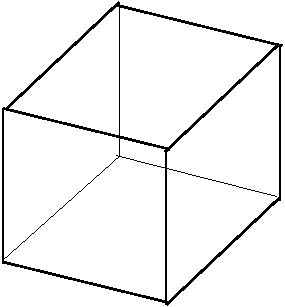
\includegraphics[width=0.30\textwidth,angle=0]{./figures_3D_Maxwell/cube.png}
\end{center}

}

%======================================================================
\frame{\frametitle{Fichera corner}
\framesubtitle{~~}

Divide it into eight smaller cubes and remove one:
\begin{center}   
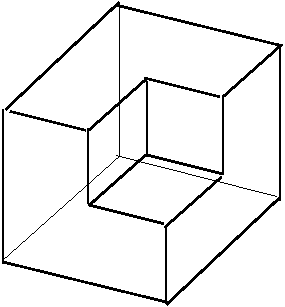
\includegraphics[width=0.30\textwidth,angle=0]{./figures_3D_Maxwell/Fichera_corner.png}
\end{center}

}

%======================================================================
\frame{\frametitle{Fichera corner microwave}
\framesubtitle{~~}

Attach a waveguide:

\begin{center}
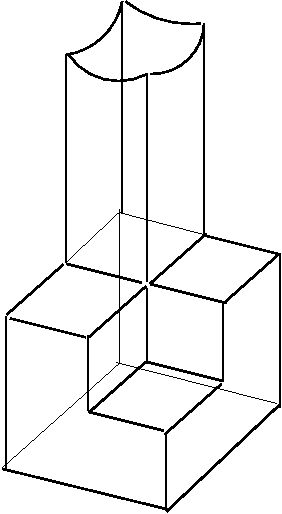
\includegraphics[width=.3\textwidth,angle=0]{./figures_3D_Maxwell/Fichera_microwave.png}
$
\begin{array}{l}
\vspace*{-4cm}
aaaa\\
\epsilon = \mu = 1, \sigma = 0\\
\omega = 5 \text{(1.6 wavelengths in the cube)}
\end{array}
$
\end{center}
Cut the waveguide and use the lowest propagating mode for BC along the cut.

}




%======================================================================
\frame{\frametitle{Fichera corner microwave, $p=2$.}
\framesubtitle{~~}



\begin{center}   
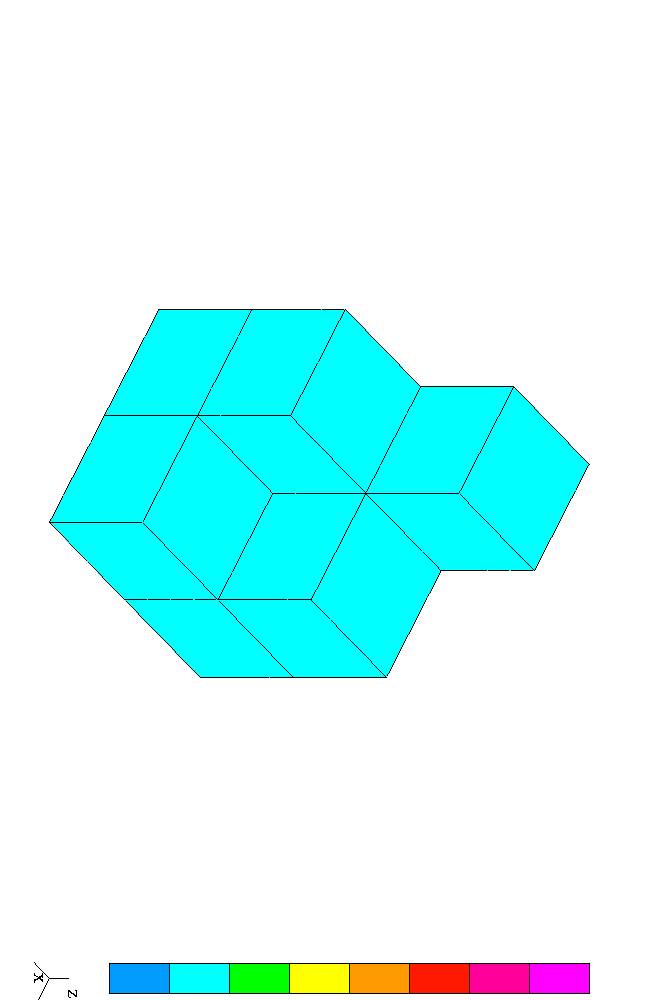
\includegraphics[width=0.30\textwidth,angle=90]{./figures_3D_Maxwell/mesh0.png}
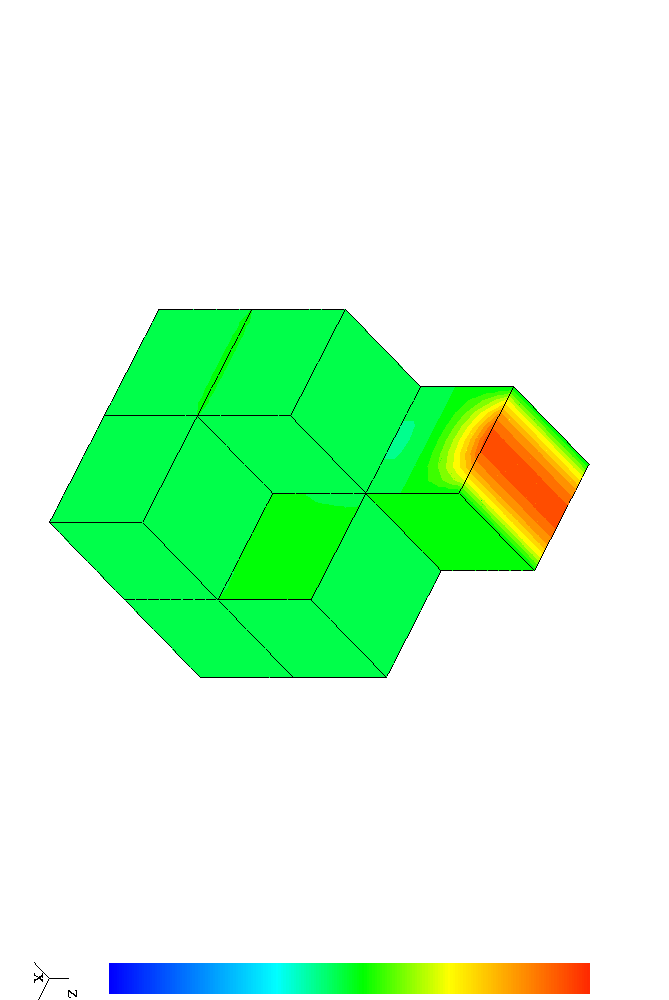
\includegraphics[width=0.30\textwidth,angle=90]{./figures_3D_Maxwell/sol0A.png}\\
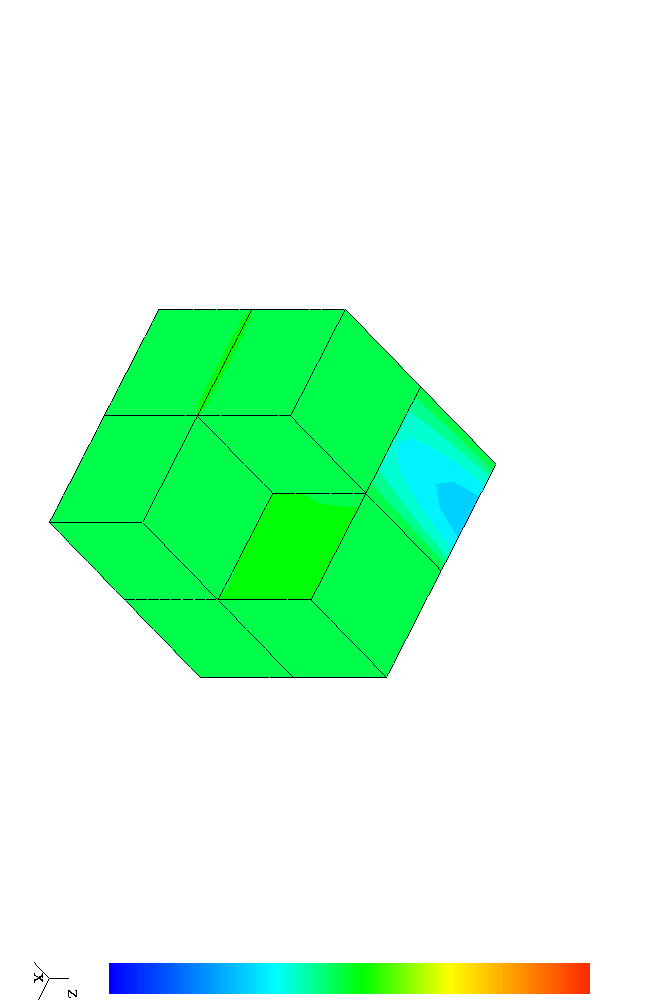
\includegraphics[width=0.30\textwidth,angle=90]{./figures_3D_Maxwell/sol0B.png}
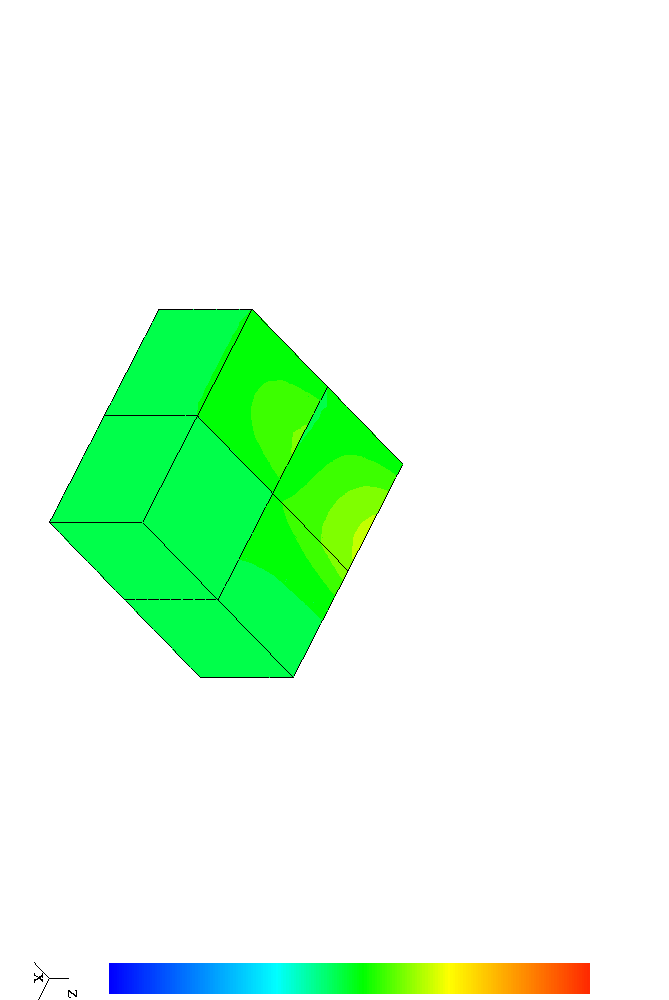
\includegraphics[width=0.30\textwidth,angle=90]{./figures_3D_Maxwell/sol0C.png}\\
Initial mesh and real part of $E_1$
\end{center}


}


%======================================================================
\frame{\frametitle{Fichera corner microwave, $p=2$.}
\framesubtitle{~~}



\begin{center}   
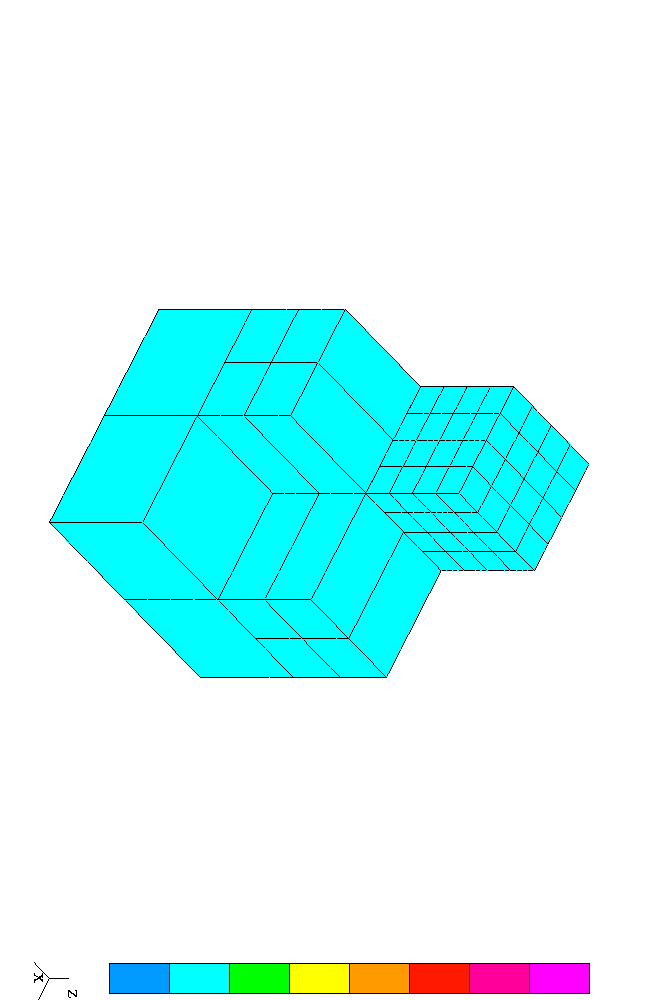
\includegraphics[width=0.30\textwidth,angle=90]{./figures_3D_Maxwell/mesh1.png}
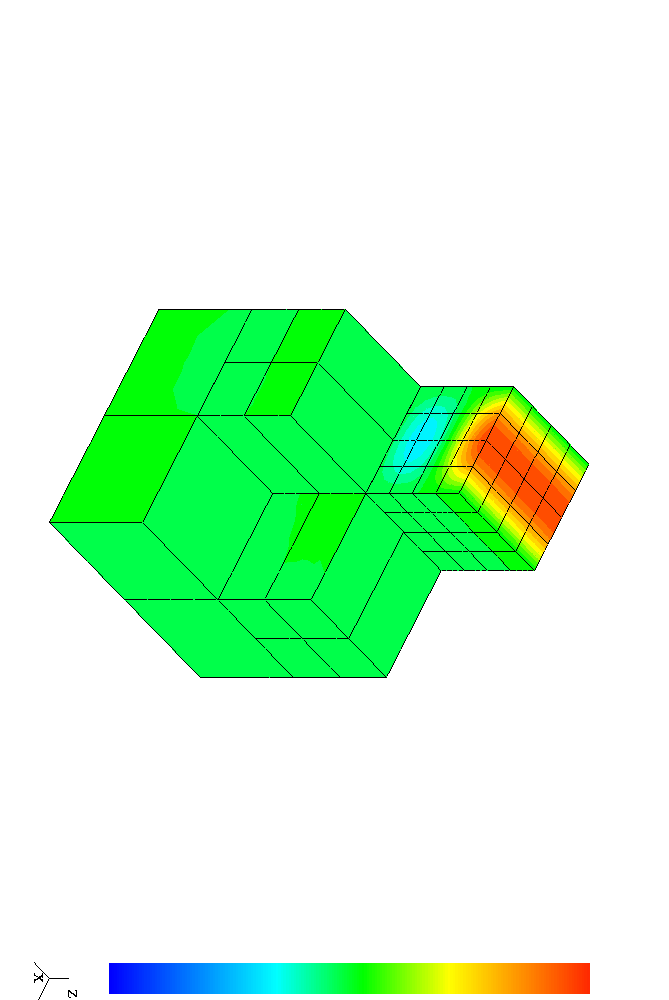
\includegraphics[width=0.30\textwidth,angle=90]{./figures_3D_Maxwell/sol1A.png}\\
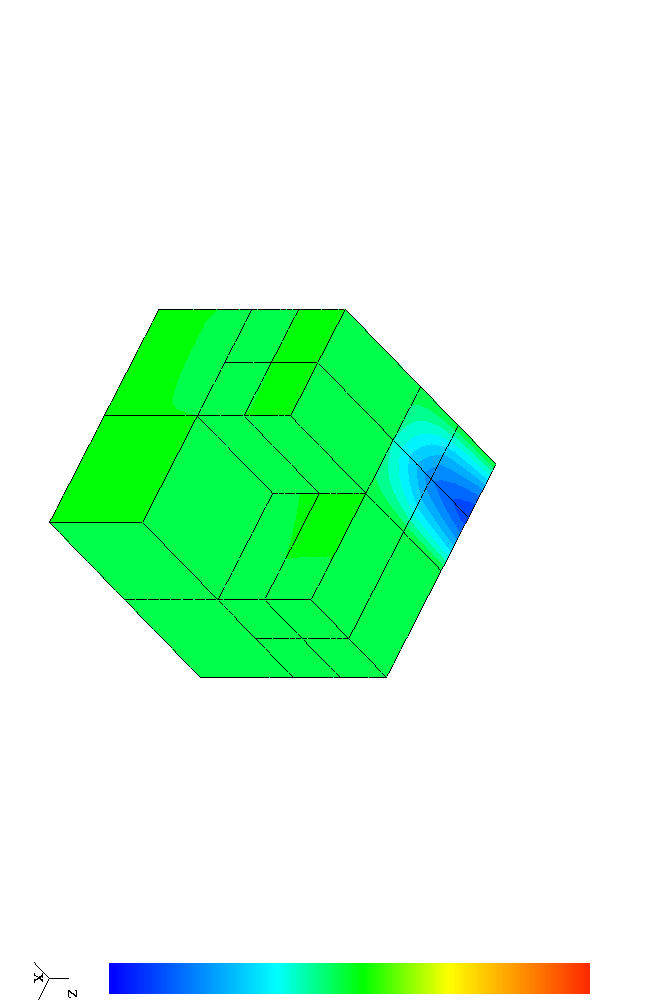
\includegraphics[width=0.30\textwidth,angle=90]{./figures_3D_Maxwell/sol1B.png}
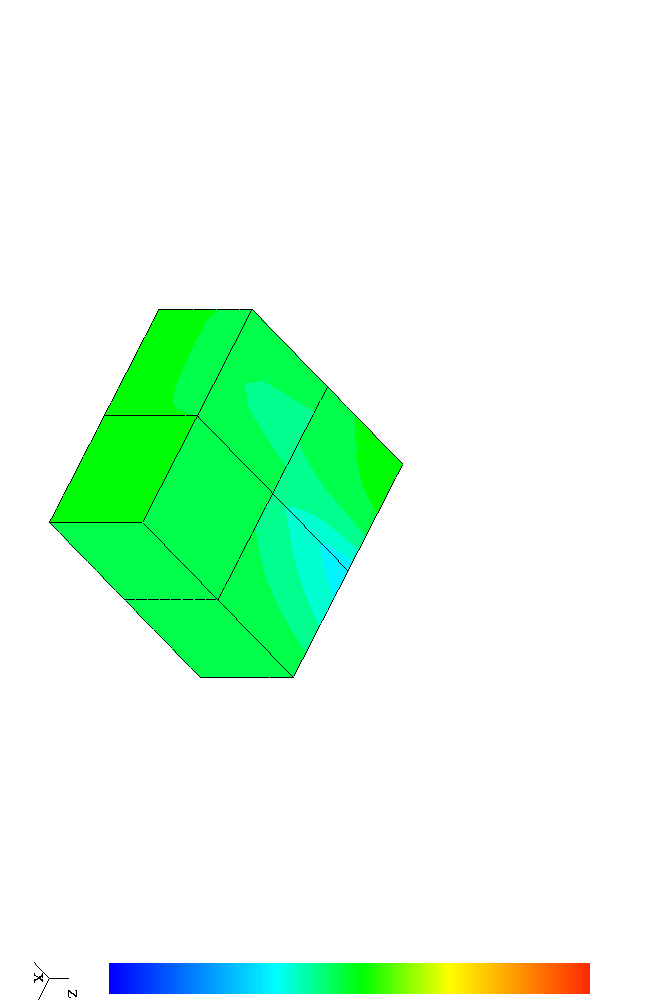
\includegraphics[width=0.30\textwidth,angle=90]{./figures_3D_Maxwell/sol1C.png}\\
Mesh and real part of $E_1$ after two refinements
\end{center}


}

%======================================================================
\frame{\frametitle{Fichera corner microwave, $p=2$.}
\framesubtitle{~~}



\begin{center}   
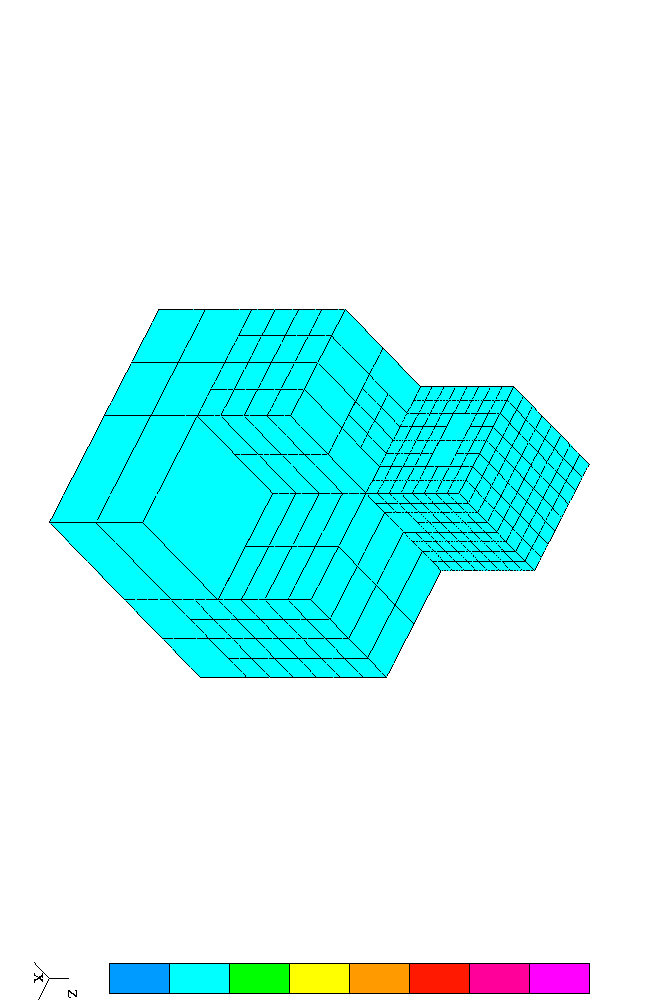
\includegraphics[width=0.30\textwidth,angle=90]{./figures_3D_Maxwell/mesh2.png}
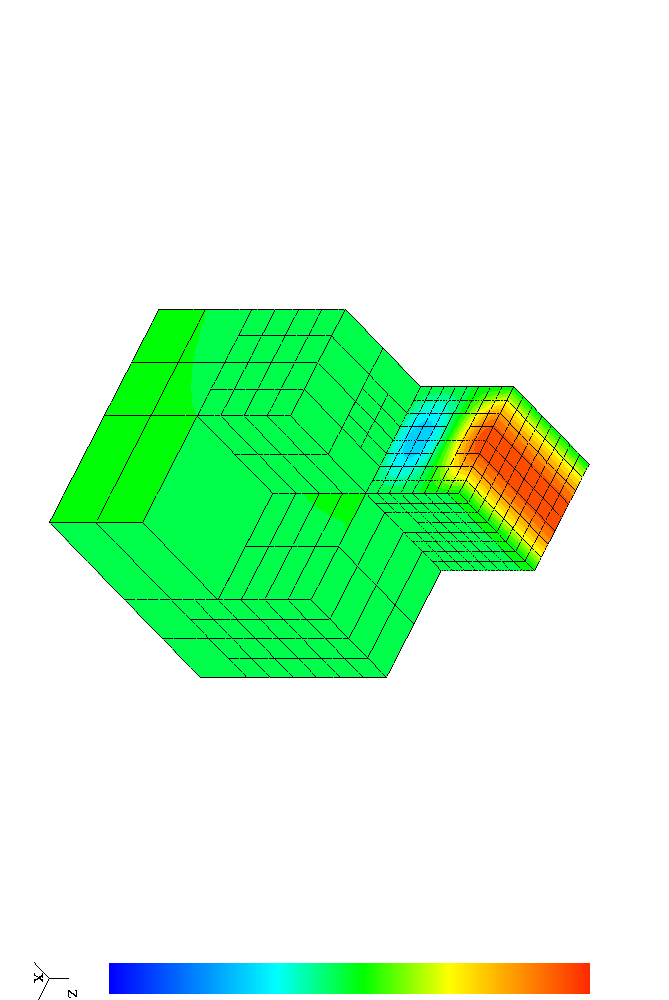
\includegraphics[width=0.30\textwidth,angle=90]{./figures_3D_Maxwell/sol2A.png}\\
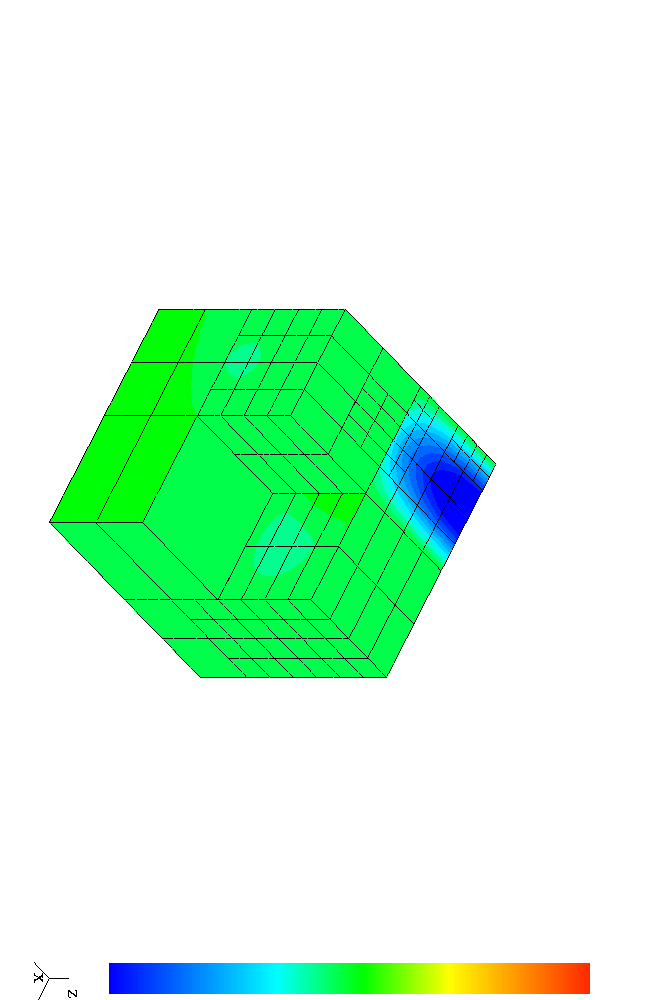
\includegraphics[width=0.30\textwidth,angle=90]{./figures_3D_Maxwell/sol2B.png}
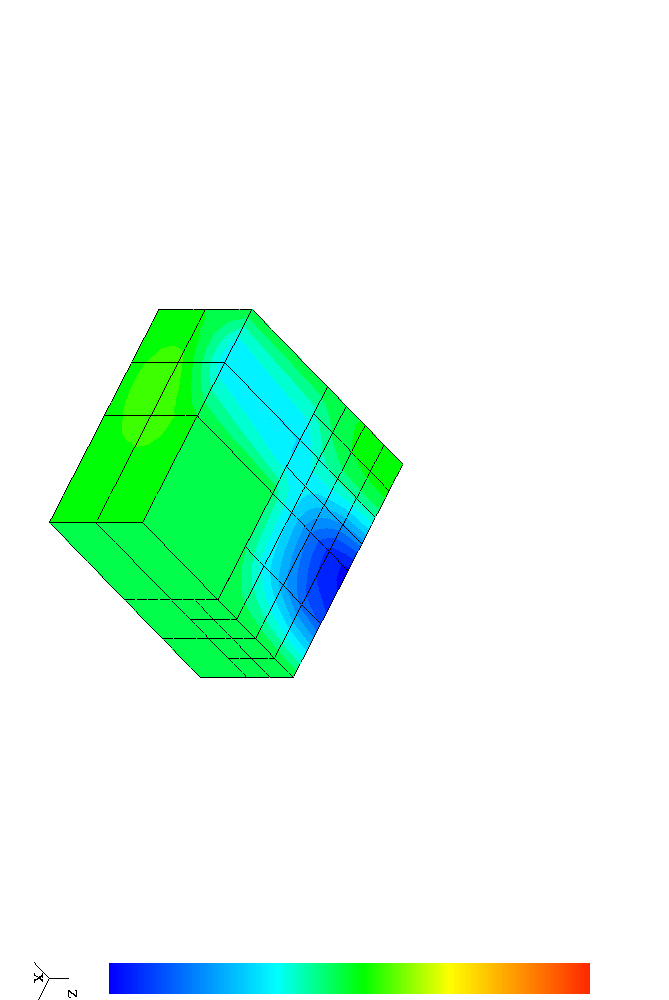
\includegraphics[width=0.30\textwidth,angle=90]{./figures_3D_Maxwell/sol2C.png}\\
Mesh and real part of $E_1$ after four refinements
\end{center}


}

%======================================================================
\frame{\frametitle{Fichera corner microwave, $p=2$.}
\framesubtitle{~~}



\begin{center}   
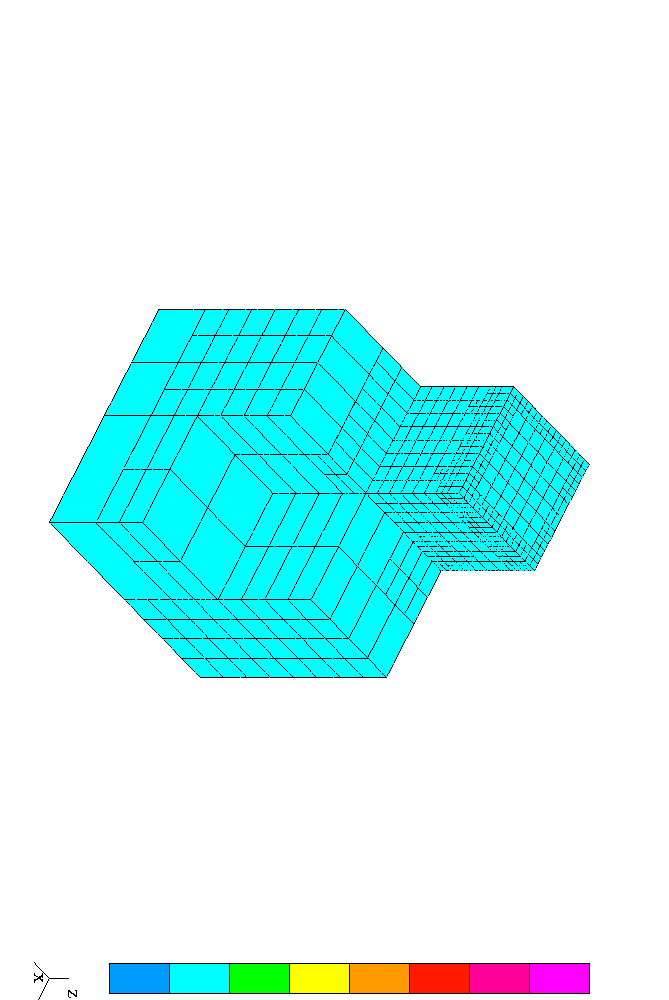
\includegraphics[width=0.30\textwidth,angle=90]{./figures_3D_Maxwell/mesh3.png}
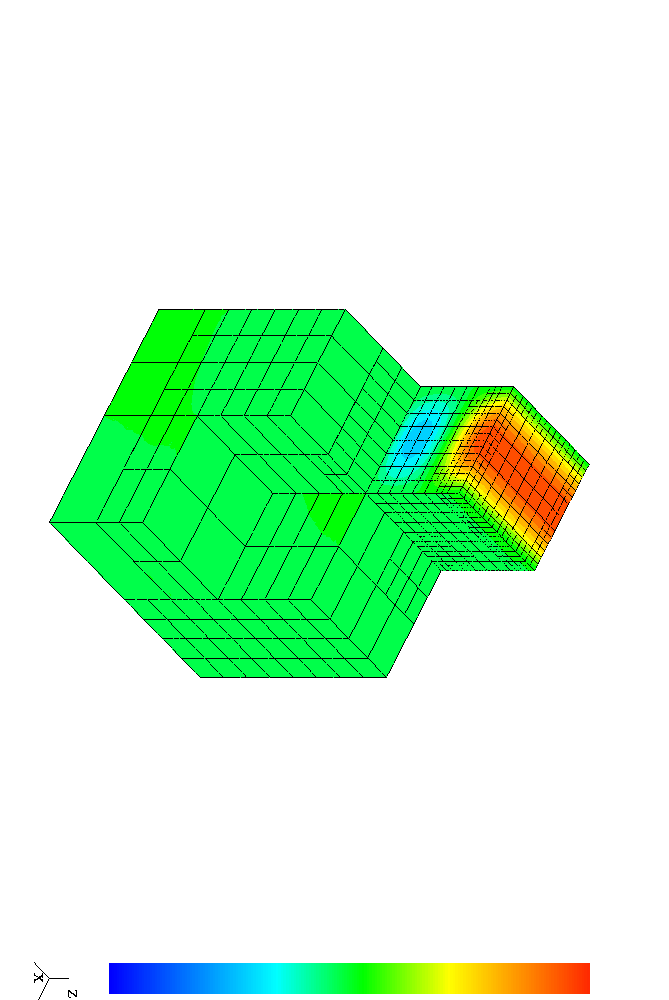
\includegraphics[width=0.30\textwidth,angle=90]{./figures_3D_Maxwell/sol3A.png}\\
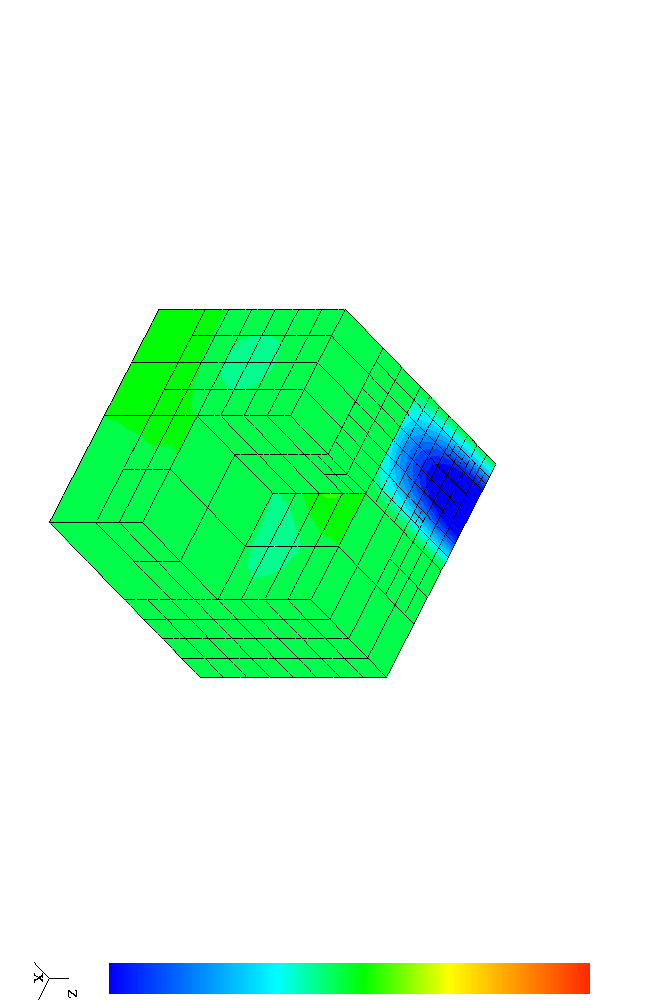
\includegraphics[width=0.30\textwidth,angle=90]{./figures_3D_Maxwell/sol3B.png}
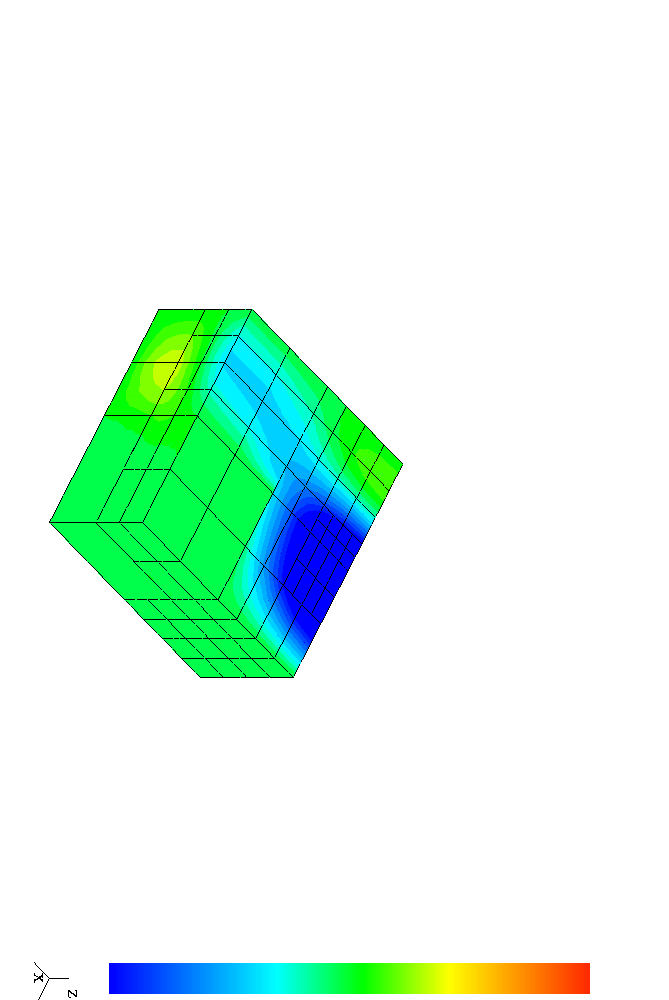
\includegraphics[width=0.30\textwidth,angle=90]{./figures_3D_Maxwell/sol3C.png}\\
Mesh and real part of $E_1$ after six refinements
\end{center}


}

%======================================================================
\frame{\frametitle{Fichera corner microwave, $p=2$.}
\framesubtitle{~~}



\begin{center}   
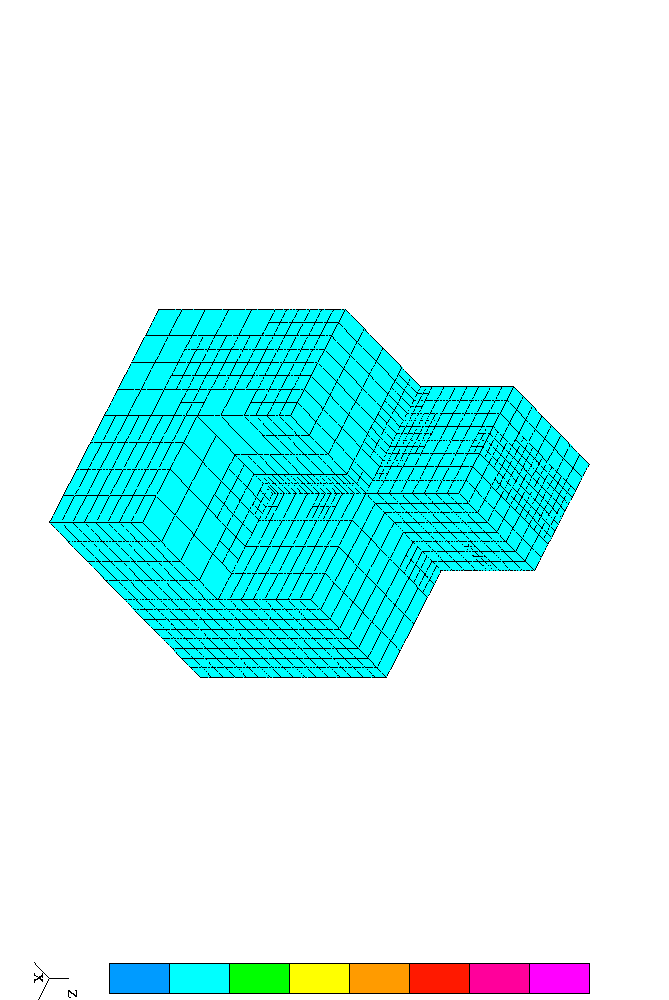
\includegraphics[width=0.30\textwidth,angle=90]{./figures_3D_Maxwell/mesh4.png}
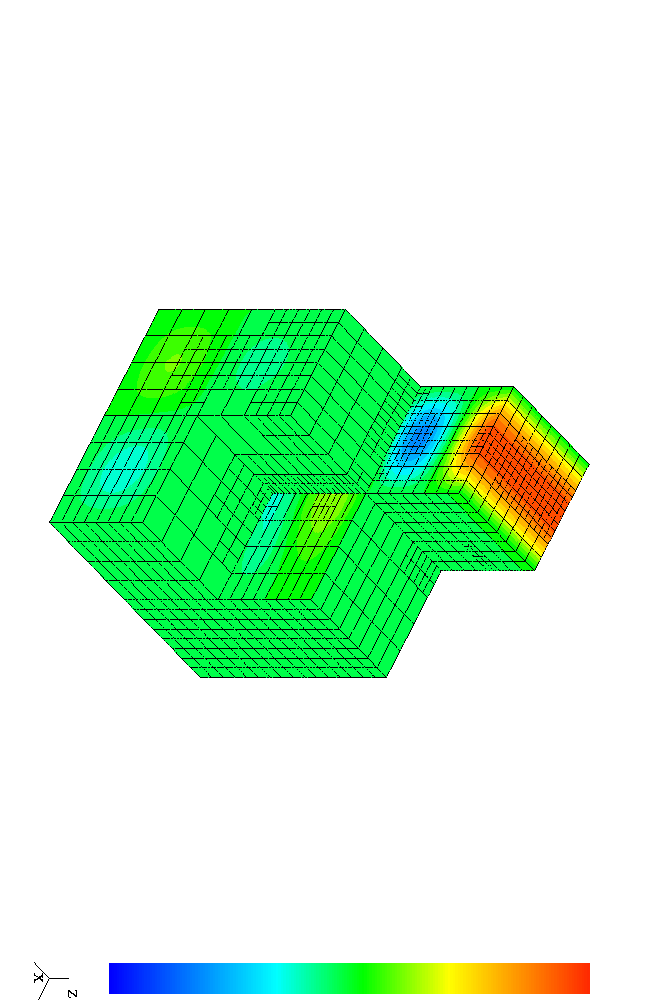
\includegraphics[width=0.30\textwidth,angle=90]{./figures_3D_Maxwell/sol4A.png}\\
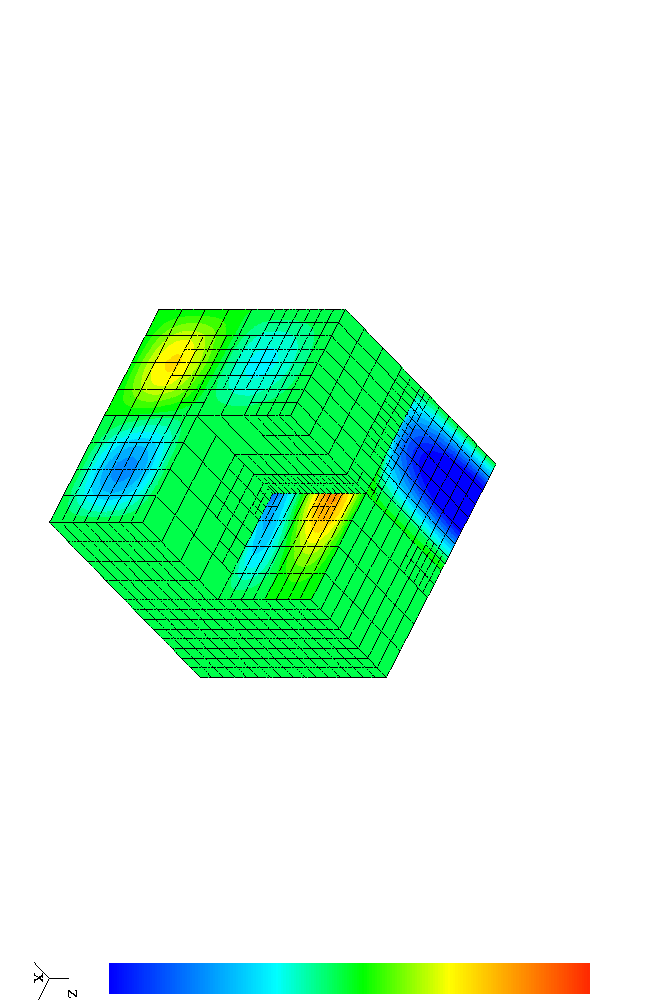
\includegraphics[width=0.30\textwidth,angle=90]{./figures_3D_Maxwell/sol4B.png}
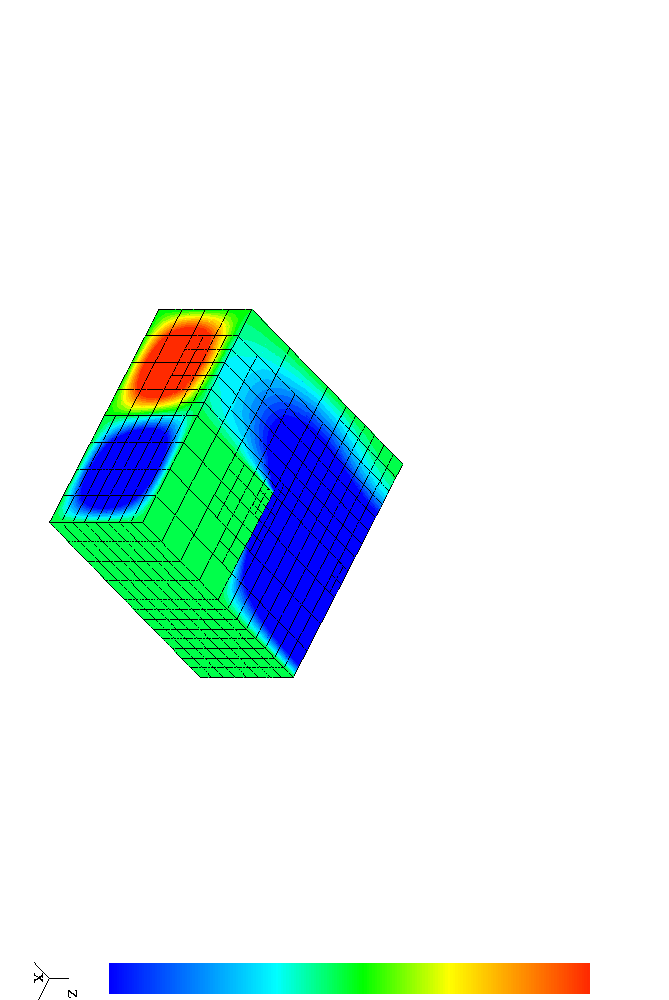
\includegraphics[width=0.30\textwidth,angle=90]{./figures_3D_Maxwell/sol4C.png}\\
Mesh and real part of $E_1$ after eight refinements
\end{center}


}


%======================================================================
\frame{\frametitle{}
\framesubtitle{~~}

\begin{center}
{\Large  \bf
From Ph.D. Dissertation of Jesse Chan:\\
Compressible Navier-Stokes Equations:\\
Carter's flat plate problem
\footnote{\tiny
L.D., J.T. Oden, W. Rachowicz, ``A New Finite Element Method for Solving Compressible 
Navier-Stokes
Equations Based on an Operator Splitting Method and $hp$ Adaptivity,'',
{\em Comput. Methods Appl. Mech. Engrg.}, {\bf 84}, 275-326, 1990.
}

}

\end{center}

\begin{figure}
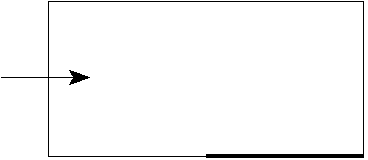
\includegraphics[scale=.3]{./figures_flat_plate/plate.png}\\
$\text{M}_\infty = 3, \text{Re}_L = 1000, \text{Pr} = 0.72, \gamma = 1.4, \theta_\infty = 390^o[\text{R}]$
\end{figure}


}







\frame{\frametitle{Extrapolation to Compressible NS Equations}
\framesubtitle{~~}

\onslide*<1>{
Initial Mesh ($p=2$):
\begin{figure}
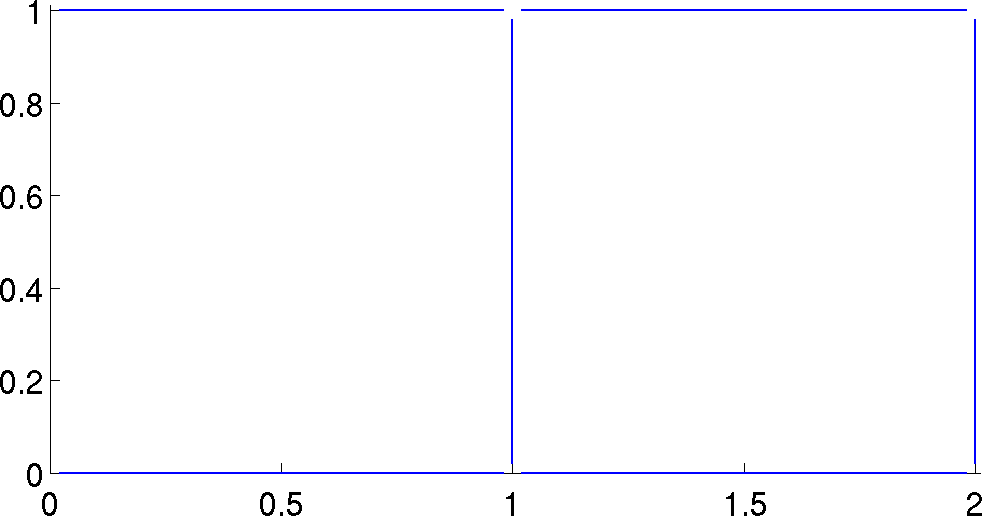
\includegraphics[width=0.2\textwidth]{./figures_flat_plate/mesh0.png}
\end{figure}

Horizontal velocity and temperature\\
\begin{figure}
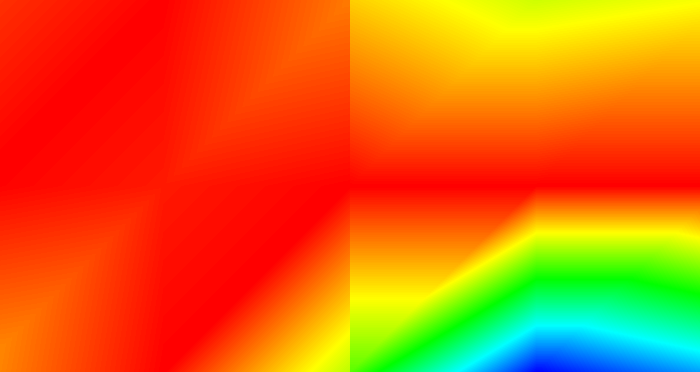
\includegraphics[width=0.45\textwidth]{./figures_flat_plate/u0.png}

\includegraphics[width=0.45\textwidth]{./figures_flat_plate/T0.png}
\end{figure}
}
\onslide*<2>{

Mesh 1:
\begin{figure}
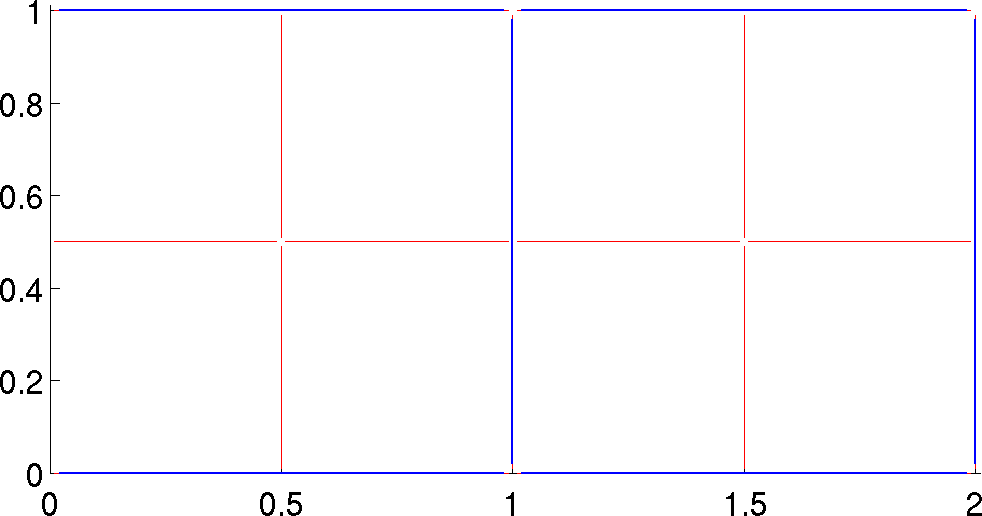
\includegraphics[width=0.2\textwidth]{./figures_flat_plate/mesh1.png}
\end{figure}

Horizontal velocity and temperature\\
\begin{figure}
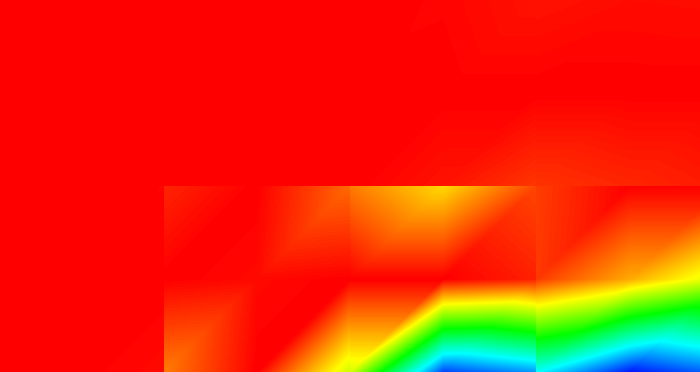
\includegraphics[width=0.45\textwidth]{./figures_flat_plate/u1.png}

\includegraphics[width=0.45\textwidth]{./figures_flat_plate/T1.png}
\end{figure}
}

\onslide*<3>{

Mesh 2:
\begin{figure}
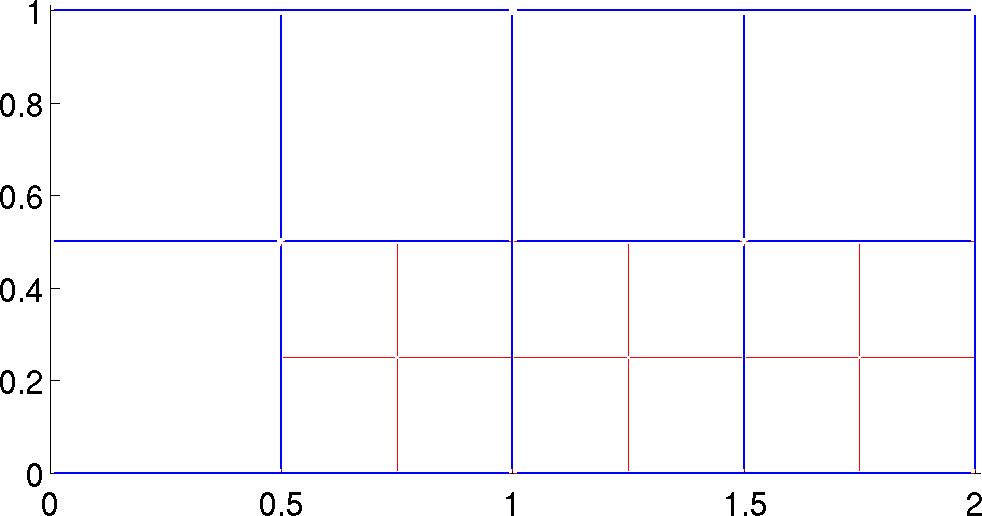
\includegraphics[width=0.2\textwidth]{./figures_flat_plate/mesh2.png}
\end{figure}

Horizontal velocity and temperature\\
\begin{figure}
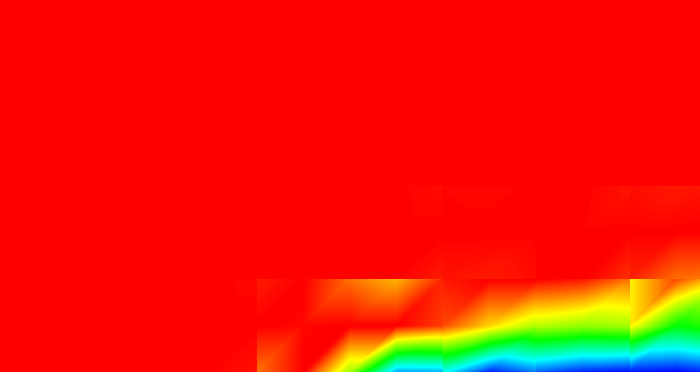
\includegraphics[width=0.45\textwidth]{./figures_flat_plate/u2.png}
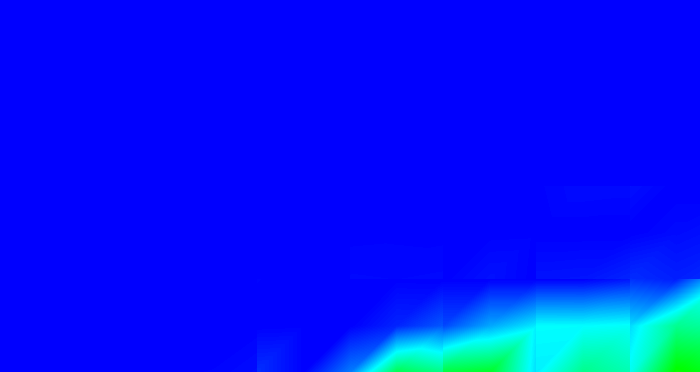
\includegraphics[width=0.45\textwidth]{./figures_flat_plate/T2.png}
\end{figure}
}


\onslide*<4>{

Mesh 3:
\begin{figure}
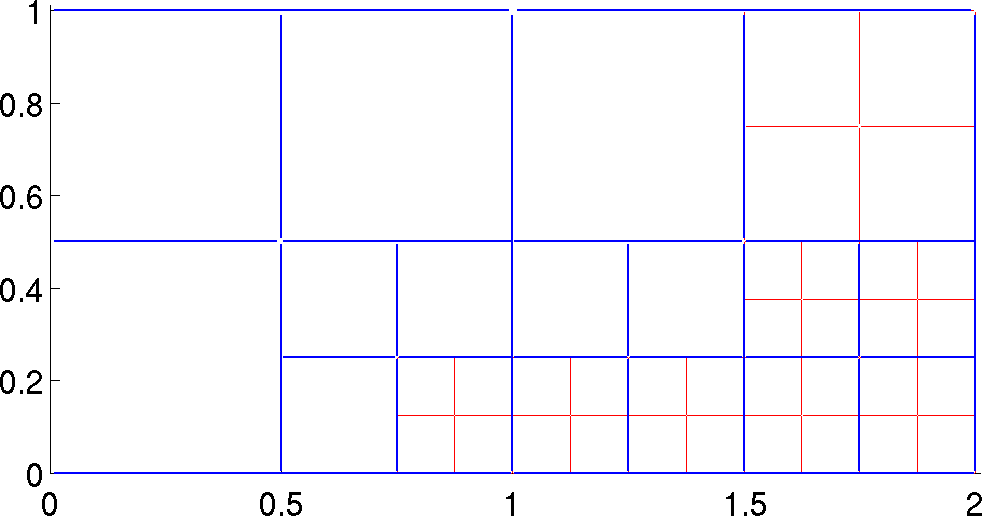
\includegraphics[width=0.2\textwidth]{./figures_flat_plate/mesh3.png}
\end{figure}

Horizontal velocity and temperature\\
\begin{figure}
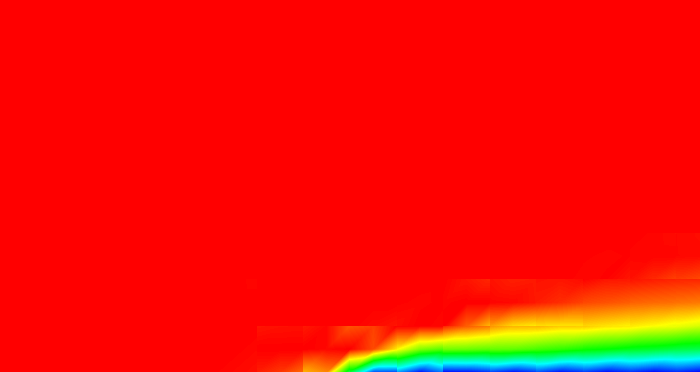
\includegraphics[width=0.45\textwidth]{./figures_flat_plate/u3.png}
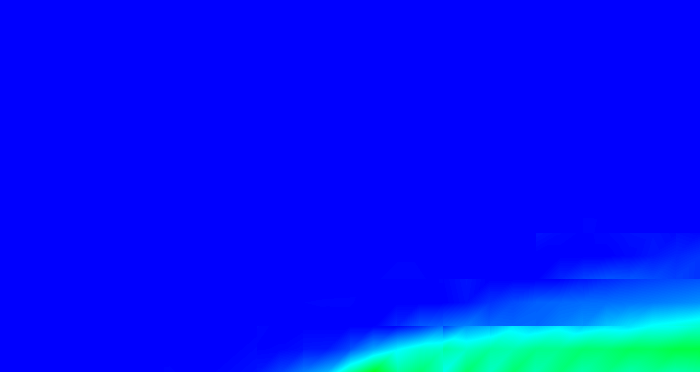
\includegraphics[width=0.45\textwidth]{./figures_flat_plate/T3.png}
\end{figure}
}

\onslide*<5>{

Mesh 4:
\begin{figure}
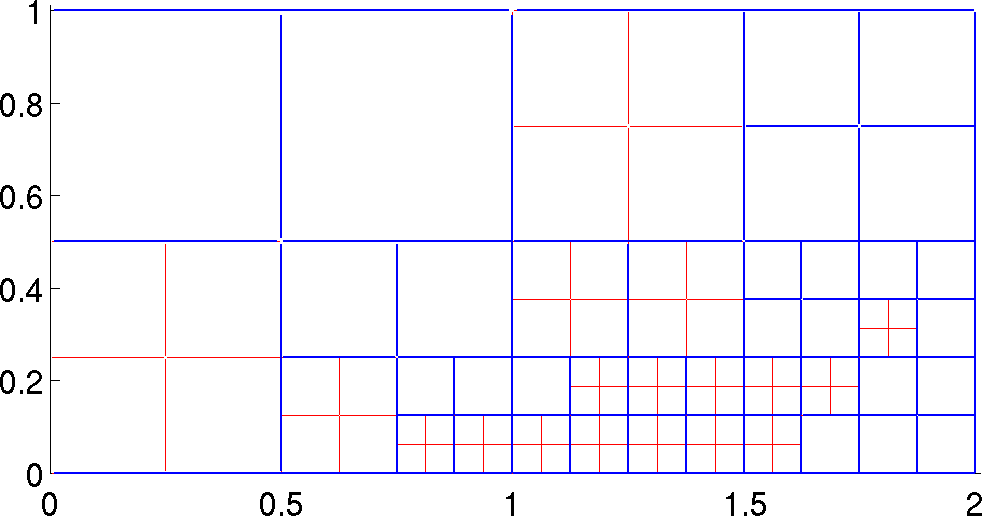
\includegraphics[width=0.2\textwidth]{./figures_flat_plate/mesh4.png}
\end{figure}

Horizontal velocity and temperature\\
\begin{figure}
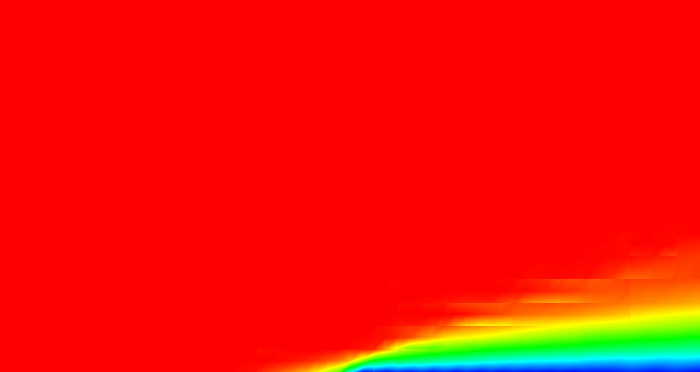
\includegraphics[width=0.45\textwidth]{./figures_flat_plate/u4.png}
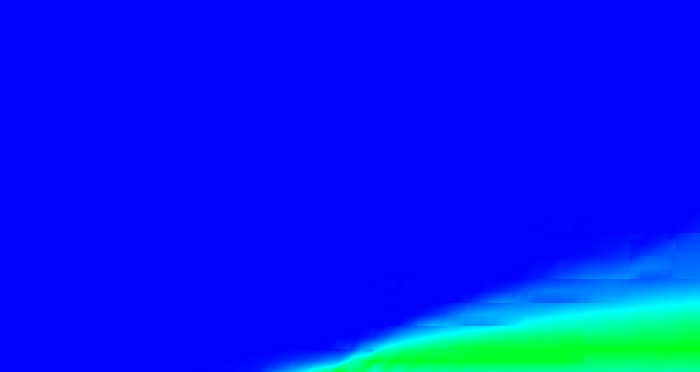
\includegraphics[width=0.45\textwidth]{./figures_flat_plate/T4.png}
\end{figure}
}

\onslide*<6>{

Mesh 5:
\begin{figure}
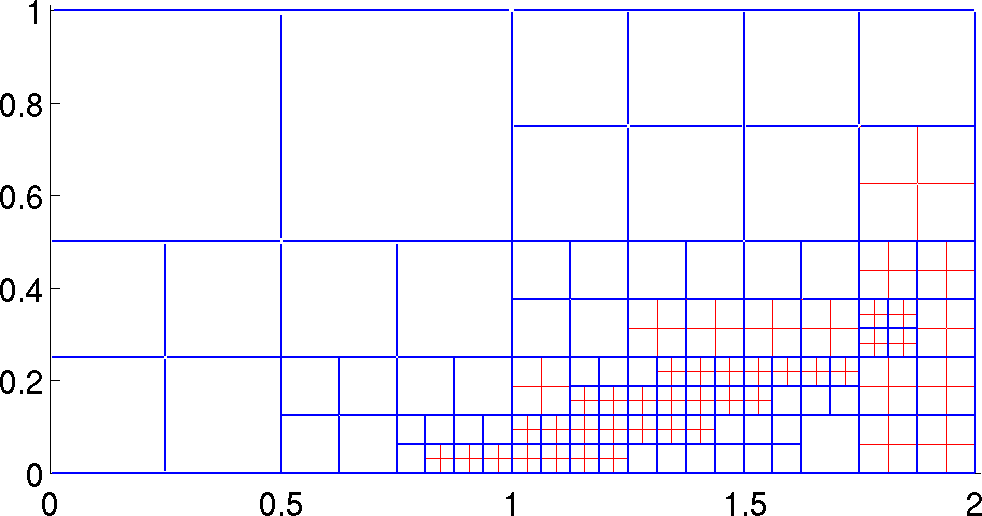
\includegraphics[width=0.2\textwidth]{./figures_flat_plate/mesh5.png}
\end{figure}

Horizontal velocity and temperature\\
\begin{figure}
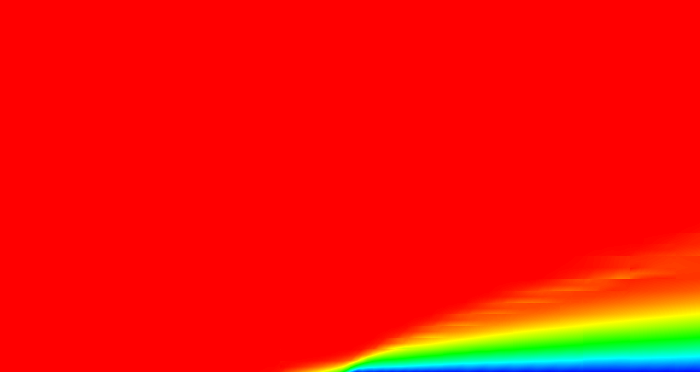
\includegraphics[width=0.45\textwidth]{./figures_flat_plate/u5.png}
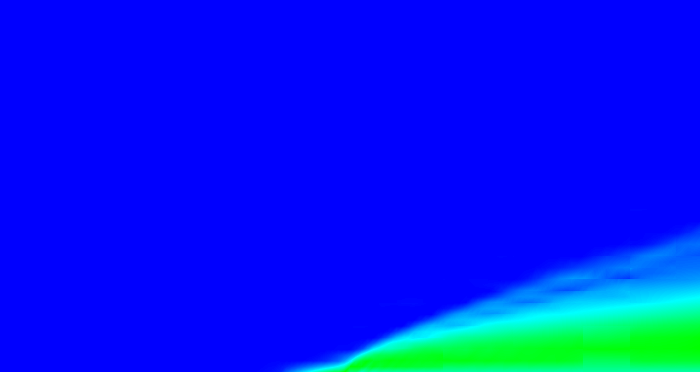
\includegraphics[width=0.45\textwidth]{./figures_flat_plate/T5.png}
\end{figure}
}


\onslide*<7>{

Mesh 7:
\begin{figure}
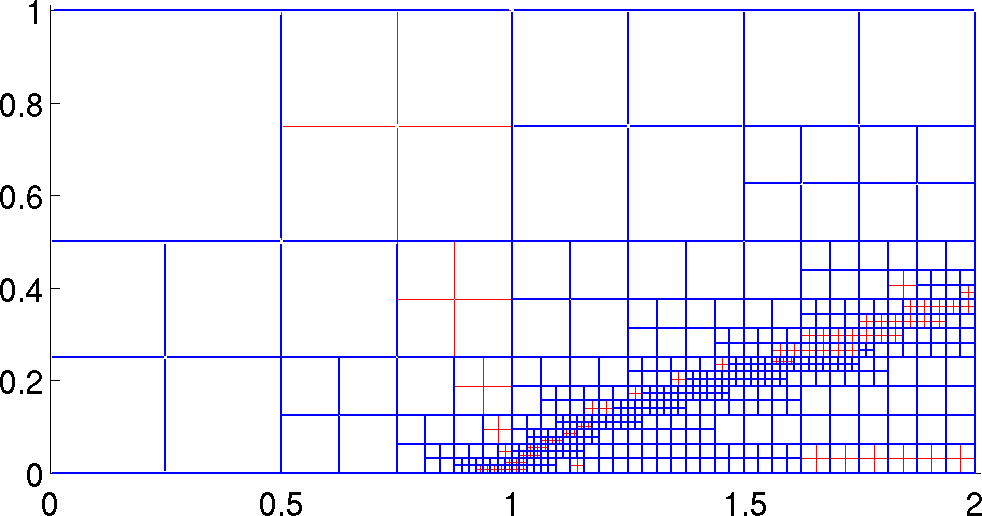
\includegraphics[width=0.2\textwidth]{./figures_flat_plate/mesh7.png}
\end{figure}

Horizontal velocity and temperature\\
\begin{figure}

\includegraphics[width=0.45\textwidth]{./figures_flat_plate/u7.png}
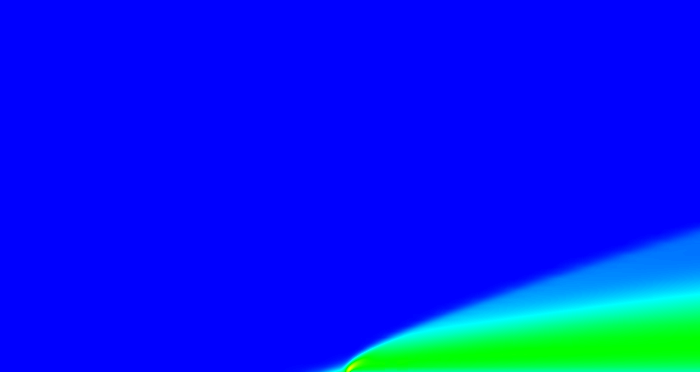
\includegraphics[width=0.45\textwidth]{./figures_flat_plate/T7.png}
\end{figure}
}

\onslide*<8>{

Mesh 8:
\begin{figure}
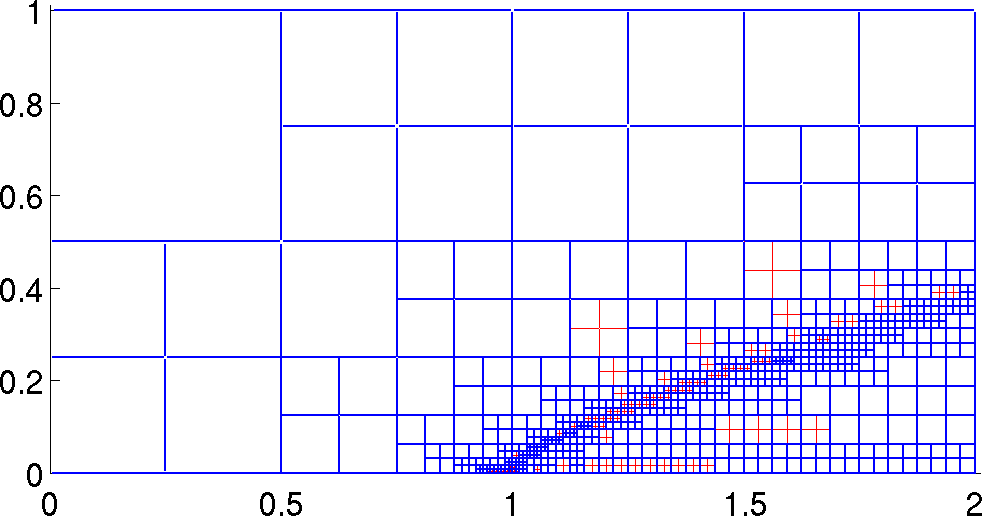
\includegraphics[width=0.2\textwidth]{./figures_flat_plate/mesh8.png}
\end{figure}

Horizontal velocity and temperature\\
\begin{figure}

\includegraphics[width=0.45\textwidth]{./figures_flat_plate/u8.png}
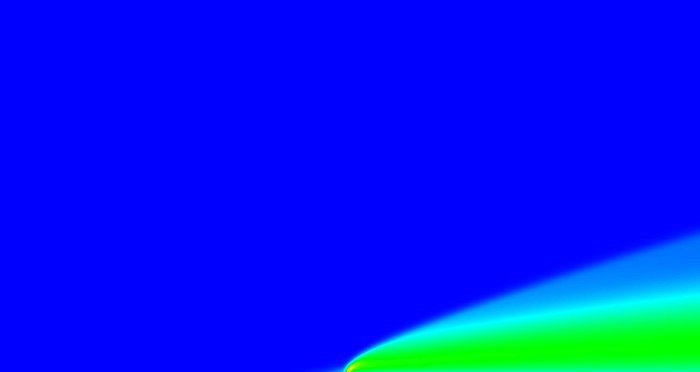
\includegraphics[width=0.45\textwidth]{./figures_flat_plate/T8.png}
\end{figure}
}

\onslide*<9>{

Mesh 9:
\begin{figure}
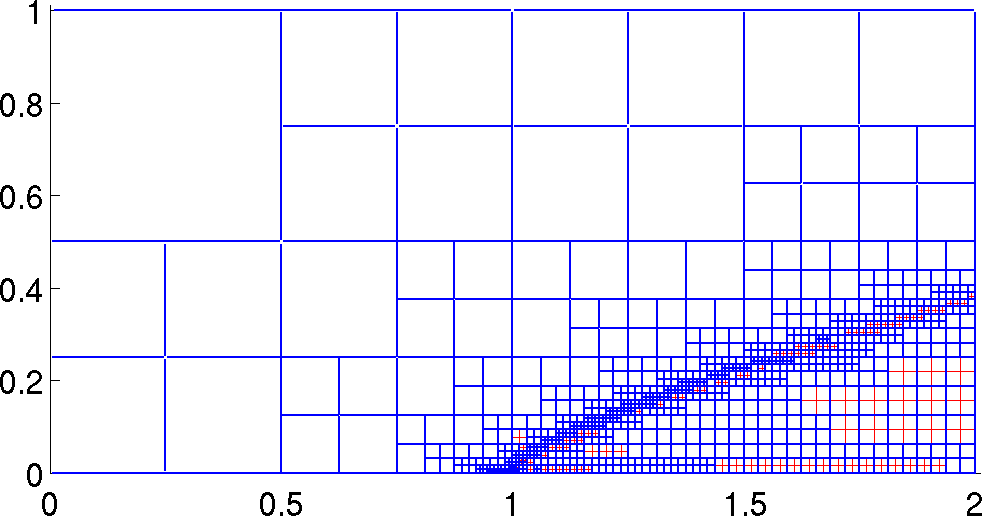
\includegraphics[width=0.2\textwidth]{./figures_flat_plate/mesh9.png}
\end{figure}

Horizontal velocity and temperature\\
\begin{figure}
\includegraphics[width=0.45\textwidth]{./figures_flat_plate/u9.png}
\includegraphics[width=0.45\textwidth]{./figures_flat_plate/T9.png}
\end{figure}
}

\onslide*<10>{

Mesh 10:
\begin{figure}
\includegraphics[width=0.2\textwidth]{./figures_flat_plate/mesh10.png}
\end{figure}

Horizontal velocity and temperature\\
\begin{figure}
\includegraphics[width=0.45\textwidth]{./figures_flat_plate/u10.png}
\includegraphics[width=0.45\textwidth]{./figures_flat_plate/T10.png}
\end{figure}
}




}


\frame{\frametitle{Extrapolation to Compressible NS Equations}
\framesubtitle{~~}

\begin{center}
\begin{figure}
\includegraphics[width=0.6\textwidth]{./figures_flat_plate/heatflux.png}
\end{figure}
Heat flux along the plate
\end{center}


}

% ------------------------------------------------------------
\frame{\frametitle{Compressible Navier-Stokes}
\framesubtitle{Sod Shock Tube with $\mu=10^{-5}$}  %% needed for proper positioning of the logo ...
\foreach \n in {1,...,15}
{
\only<\n>
{
\vspace{-2ex}

% \begin{minipage}[c]{0.45\linewidth}
\begin{figure}[ht]
\centering
\includegraphics[height=0.4\textwidth]{figures_spacetime/den\n.pdf}
\end{figure}
% \end{minipage}
% \begin{minipage}[c]{0.45\linewidth}
% \includegraphics[height=0.3\textwidth]{figures_spacetime/vel\n.pdf}\\
% \end{minipage}
% \begin{minipage}[c]{0.45\linewidth}
% \includegraphics[height=0.3\textwidth]{figures_spacetime/pres\n.pdf}
% \end{minipage}
% \begin{minipage}[c]{0.45\linewidth}
\begin{figure}[ht]
\centering
\includegraphics[width=0.6\textwidth]{figures_spacetime/mesh\n.png}
\end{figure}
% \end{minipage}
}
}
}

%======================================================================
% \frame{\frametitle{Punchline 2}
% \framesubtitle{~~}

% \begin{center}
% {\Large You can control the norm in which you want to converge.


% }

% \end{center}

% }


\section{You can control the norm in which you want to converge.}




%======================================================================
\frame{\frametitle{}
\framesubtitle{~~}
\begin{center}

{\Large \bf The simplest singular perturbation problem:\\[8pt]
reaction-dominated diffusion
\footnote{\small L.D. and I. Harari, ``Primal DPG Method for Reaction dominated Diffusion'', in preparation.}

}
\end{center}



}






%======================================================================
\frame{\frametitle{The simplest singular perturbation problem: Reaction-dominated diffusion}
\framesubtitle{~~}
$$
\left\{
\begin{array}{rll}
u & = 0 & \text{ on } \Gamma\\
- \epsilon^2 \Delta u + c(x) u & = f & \text{ in } \Omega
\end{array}
\right.
$$
where $0 < c_0 \leq c(x) \leq c_1$.

Standard variational formulation:
$$
\left\{
\begin{array}{l}
u \in H^1(\Omega) \\[8pt]
\epsilon^2 (\bfnab u, \bfnab v) + (cu,v) = (f,v) \quad v \in H^1(\Omega)
\end{array}
\right.
$$
Standard Galerkin method delivers the best approximation error in the energy norm:
$$
\Vert u \Vert_{\epsilon^k}^2 := \epsilon^k \Vert \bfnab u \Vert^2 + \Vert c^{1/2} u \Vert^2, \quad k=2
$$

}


%======================================================================
\frame{\frametitle{Convergence in ``balanced'' norm}
\framesubtitle{~~}

{\bf Fact:} Under favorable regularity conditions, the solution is {\em uniformly}
bounded in data $f$ in a ``balanced'' norm
\footnote{\tiny R.~Lin and M.~Stynes, ``A balanced finite element method for singularly perturbed
  reaction-diffusion problems'',
{\em SIAM J. Numer. Anal.}, {\bf 50(5):} 2729--2743, 2012.}
:
$$
\Vert u \Vert_{\epsilon}^2 := \textcolor{red}{\epsilon} \Vert \bfnab u \Vert^2 + \Vert c^{1/2} u \Vert^2
$$
i.e.
$$
\Vert u \Vert_{\epsilon} \lesssim \Vert f \Vert_{\text{appropriate}}
$$
{\bf Question:} Can we select the test norm in such a way that the DPG method
will be {\em robust} in the balanced norm ?
$$
\Vert u - u_h \Vert_\epsilon + \Vert \hat{t} - \hat{t}_h \Vert_?
\lesssim \inf_{w_h}\Vert u - w_h \Vert_\epsilon + \inf_{\hat{r}_h}\Vert \hat{t} - \hat{r}_h \Vert_? 
$$


}


%======================================================================
\frame{\frametitle{A bit of history: 
\framesubtitle{Optimal test functions of Barret and Morton
\footnote{
\tiny 
\begin{itemize}
  \item J.W. Barret and K. W. Morton, 
``Approximate Symmetrization and Petrov-Galerkin Methods for 
Diffusion-Convection Problems'', 
{\em Comp. Meth. Appl. Mech and Engng.}, 
{\bf 46}, 97 (1984).
  \item L. D. and J. T. Oden, 
``An Adaptive Characteristic {Petrov-Galerkin} Finite Element 
                  Method for Convection-Dominated Linear and Nonlinear 
                  Parabolic Problems in One Space Variable'', 
{\em Journal of Computational Physics}, {\bf 68(1):} 188--273, 1986.
\end{itemize}
}}
}

For each $w \in U_h$, determine the corresponding $v_w$ that solves the
auxiliary variational problem:
$$
\left\{
\begin{array}{l}
v_w \in H^1_0(\Omega) \\[8pt]
\underbrace{\epsilon^2 (\bfnab \delta u, \bfnab v_w) + (c \, \delta u, v_w )}_
{\text{the bilinear form we have}}
= \underbrace{\epsilon (\bfnab \delta u, w) + (c \, \delta u, w )}_{
\text{the bilinear form we want}}
\quad \forall \delta u \in H^1_0(\Omega)
\end{array}
\right.
$$
With the optimal test functions, the Galerkin orthogonality for the original form
changes into Galerkin orthogonality in the desired, ``balanced'' norm:
{\small 
$$
\epsilon^2 (\bfnab (u - u_h), \bfnab v_w) + (c \, (u - u_h), v_w ) = 0 
\quad \implies
\textcolor{red}{\epsilon} (\bfnab (u - u_h), \bfnab v_u) + (c \, (u - u_h), w ) = 0 
$$
}
Consequently, the PG solution delivers the best approximation error in the
desired norm.

}


%======================================================================
\frame{\frametitle{Constructing optimal test norm
\framesubtitle{~~}
\footnote{\tiny L. D., M. Heuer,
``Robust  DPG  Method for Convection-Dominated Diffusion Problems,''
{\em SIAM J. Num. Anal}, {\bf 51:} 2514--2537, 2013. }
}
{\small 
\begin{theorem}
Let $v_u$ be the Barret-Morton optimal test function corresponding to $u$.
Let $\Vert v_u \Vert_V$ be a test norm such that
$$
\Vert v_u \Vert_V \lesssim  \Vert u \Vert_{\epsilon}
$$
Then
$$
\Vert u - u_h \Vert_{\epsilon} \lesssim \Vert  u - u_h \Vert_E
= \inf_{w_h \in U_h} \Vert  u - w_h \Vert_E \leq \text{BAE estimate}
$$
\end{theorem}
{\bf Proof:}
$$
\begin{array}{lll}
\Vert u \Vert_{\epsilon}^2 & = \epsilon (\bfnab u,\bfnab u) + (cu,u) 
 = \epsilon^2 (\bfnab u,\bfnab v_u) + (cu,v_u) \\[8pt]
& = b((u,\hat{t}), v_u) 
\leq \frac{  b((u,\hat{t}), v_u)  }{\Vert v_u \Vert_V} \, \Vert v_u \Vert_V \\[8pt]
& \leq \sup_v \frac{   b((u,\hat{t}), v_u)             }{\Vert v \Vert_V} \, \Vert v_u \Vert_V 
 = \Vert (u,\hat{t}) \Vert_E \, \Vert v_u \Vert_V \\[8pt]
& \lesssim  \Vert (u,\hat{t}) \Vert_E \, \Vert u \Vert_{\epsilon}
\end{array}
$$
}

}

%======================================================================
\frame{\frametitle{Constructing optimal test norm}
\framesubtitle{~~}
{\bf The point:} Construction of the optimal test norm is reduced to the stability
(robustness) 
analysis for the Barret-Morton test functions.
\begin{lemma}
Let
$$
  \Vert v \Vert_V^2 :=  \textcolor{red}{\epsilon^3}  \Vert \bfnab v \Vert^3 +  \Vert c^{1/2} v \Vert^2
$$
Then
$$
\Vert v_u \Vert \lesssim  \Vert u \Vert_{\epsilon}
$$
\end{lemma}
In order to avoid boundary layers in the optimal test functions (that we cannot resolve
using simple enriched space) we scale the reaction term with a mesh-dependent factor:
$$
  \Vert v \Vert_{V,mod}^2 :=  \epsilon^3  \Vert \bfnab v \Vert^3 +  
\textcolor{red}{\min\{1,\frac{\epsilon^3}{h^2}\}}
\Vert c^{1/2} v \Vert^2
$$


}

%======================================================================
\frame{\frametitle{Manufactured solution of Lin and Stynes, $\epsilon = 10^{-1}$}
\framesubtitle{~~}


\begin{center}   
\includegraphics[width=0.5\textwidth,angle=90]{./figures_2D_reaction_diffusion/Stynes_solution.png}\\[8pt]
The functions exhibits strong boundary layers invisible in this scale.\\[8pt]
Range: (-0.6,0.6)
\end{center}



}


%======================================================================
\frame{\frametitle{Manufactured solution of Lin and Stynes, $\epsilon = 10^{-1}$}
\framesubtitle{~~}


\begin{center}   
\includegraphics[width=0.5\textwidth,angle=90]{./figures_2D_reaction_diffusion/zoom_on_north_boundary_layer.png}\\[8pt]
Zoom on the north boundary layer.
\end{center}



}

%======================================================================
\frame{\frametitle{Optimal mesh for $\epsilon = 10^{-1}$}
\framesubtitle{~~}


\begin{center}   
\includegraphics[width=0.5\textwidth,angle=90]{./figures_2D_reaction_diffusion/optimal_mesh.png}\\[8pt]
Optimal $h$-adaptive mesh and numerical solution for $\epsilon = 10^{-1}$
\end{center}



}



%======================================================================
\frame{\frametitle{Lin/Stynes example, $\epsilon = 1$}
\framesubtitle{~~}



\begin{center}   
\includegraphics[width=0.5\textwidth,angle=90]{./figures_2D_reaction_diffusion/r0.png}\\
Residual and ``balanced'' error of $u$ for $h$-adaptive solution, $p=2$ 
\end{center}



}
%======================================================================
\frame{\frametitle{Lin/Stynes example, $\epsilon = 10^0, 10^{-1}$}
\framesubtitle{~~}



\begin{center}   
\includegraphics[width=0.5\textwidth,angle=90]{./figures_2D_reaction_diffusion/r1.png}\\
Residual and ``balanced'' error of $u$ for $h$-adaptive solution, $p=2$
\end{center}


}
%======================================================================
\frame{\frametitle{Lin/Stynes example, $\epsilon = 10^0, 10^{-1}, 10^{-2}$.}
\framesubtitle{~~}



\begin{center}   
\includegraphics[width=0.5\textwidth,angle=90]{./figures_2D_reaction_diffusion/r2.png}\\
Residual and ``balanced''  error of $u$ for $h$-adaptive solution, $p=2$
\end{center}


}
%======================================================================
\frame{\frametitle{Lin/Stynes example, $\epsilon = 10^0, 10^{-1}, 10^{-2}, 10^{-3}$.}
\framesubtitle{~~}


\begin{center}   
\includegraphics[width=0.5\textwidth,angle=90]{./figures_2D_reaction_diffusion/r3.png}\\
Residual and ``balanced'' error of $u$ for $h$-adaptive solution, $p=2$
\end{center}


}
%======================================================================
\frame{\frametitle{Lin/Stynes example, $\epsilon = 10^0, 10^{-1}, 10^{-2}, 10^{-3}, 10^{-4}$.}
\framesubtitle{~~}


\begin{center}   
\includegraphics[width=0.5\textwidth,angle=90]{./figures_2D_reaction_diffusion/r4.png}\\
Residual and ``balanced''   error of $u$ for $h$-adaptive solution, $p=2$
\end{center}


}


%======================================================================
\frame{\frametitle{Other tricks we can play: zooming on the solution}
\framesubtitle{~~}


{\bf Question:} Can we select the test norm in such a way that the DPG method
would deliver high accuracy in a preselected subdomain, e.g. $(0,\half)^2 \subset (0,1)^2$ ?

{\bf Answer:} Yes!
\begin{center}   
\includegraphics[width=0.3\textwidth,angle=90]{./figures_2D_reaction_diffusion/locally_optimal_mesh.png}
\includegraphics[width=0.3\textwidth,angle=90]{./figures_2D_reaction_diffusion/error.png}\\[8pt]
Optimal mesh and the corresponding pointwise error (range $(-0.001 - 0.001)$.
\end{center}


}



%======================================================================
% \frame{\frametitle{Punchline 3}
% \framesubtitle{~~}

% \begin{center}
% {\Large DPG is easy to code.



% }

% \end{center}

% }



\section{DPG is easy to code.}



%======================================================================
\frame{\frametitle{Other Applications
\framesubtitle{~~}
}
\bit
  \item<1->  Wave propagation problems (sonars, full wave form inversion in geomechanics, cloaking)
  \item<2->  Elasticity, shells (volumetric, shear, membrane locking)
  \item<3->  Metamaterials
\eit

}

\end{document}
